\chapter{Finite state machines} \label{ch:FSM}
\chapterquote{Darkness can not be dispelled by darkness, but by brightness. Hatred can not be overcome by hatred, but by loving kindness.}{Buddha}

\graphicspath{{Chapters/FSM/Figures/}}
\lstinputpath{Codes-Verilog/Chapter-Finite-state-machines/VerilogCodes} %path is defined in mypreamble


\section{Introduction}
In previous chapters, we saw various examples of the combinational circuits and sequential circuits. In combinational circuits, the output depends on the current values of inputs only; whereas in sequential circuits, the output depends on the current values of the inputs along with the previously stored information. In the other words, storage elements, e.g. flip flogs or registers, are required for sequential circuits. 

The information stored in the these elements can be seen as the states of the system. If a system transits between finite number of such internal states, then finite state machines (FSM) can be used to design the system. In this chapter, various finite state machines along with the examples are discussed. Further, please see the SystemVerilog-designs in Chapter \ref{ch:SystemVerilogSyn}, which provides the better ways for creating the FSM designs as compared to Verilog. 

\section{Comparison: Mealy and Moore designs}\label{sec:MealyMooreDesign}
FMS design is known as Moore design if the output of the system depends only on the states (see Fig. \ref{fig:MooreEdgeDetector}); whereas it is known as Mealy design if the output depends on the states and external inputs (see Fig. \ref{fig:MealyEdgeDetector}). Further, a system may contain both types of designs simultaneously.

\begin{noNumBox}
	Following are the differences in Mealy and Moore design, 
	\begin{enumerate}
		\item In Moore machine, the outputs depend on states only, therefore it is `\textbf{synchronous machine}' and the output is available after 1 clock cycle as shown in Fig. \ref{fig:edgeDetectorWave}. Whereas, in Mealy machine output depends on states along with external inputs; and the output is available as soon as the input is changed therefore it is `\textbf{asynchronous machine}'\footnote{See Fig. \ref{fig:Mealy_MooreGlitchFree} for more details}.
		\item Mealy machine requires fewer number of states as compared to Moore machine as shown in Fig. \ref{fig:MealyMooreDect}. 	
		\item Moore machine should be preferred for the designs, where glitches\footnote{see Section \ref{sec:glitches}} are not the problem in the systems. 
		\item Mealy machines are good for synchronous systems which requires `delay-free and glitch-free' system\footnote{See example in Section \ref{sec:exampleRegularMMGlitchFree}}, but careful design is required for asynchronous systems. Therefore, Mealy machine can be complex as compare to Moore machine. 
	\end{enumerate}
\end{noNumBox}	

\section{Example: Rising edge detector}
Rising edge detector generates a tick for the duration of one clock cycle, whenever input signal changes from 0 to 1. In this section, state diagrams of rising edge detector for Mealy and Moore designs are shown. Then rising edge detector is implemented using Verilog code. Also, outputs of these two designs are compared. 

\subsection{State diagrams: Mealy and Moore design}
Fig. \ref{fig:MealyEdgeDetector} and \ref{fig:MooreEdgeDetector} are the state diagrams for Mealy and Moore designs respectively. In Fig. \ref{fig:MealyEdgeDetector}, the output of the system is set to 1, whenever the system is in the state `zero' and value of the input signal `level' is 1; i.e. output depends on both the state and the input. Whereas in Fig. \ref{fig:MooreEdgeDetector}, the output is set to 1 whenever the system is in the state `edge' i.e. output depends only on the state of the system. 

\begin{figure}[h!]
	\centering
	\begin{subfigure}[!t]{0.45\textwidth}
		\centering
		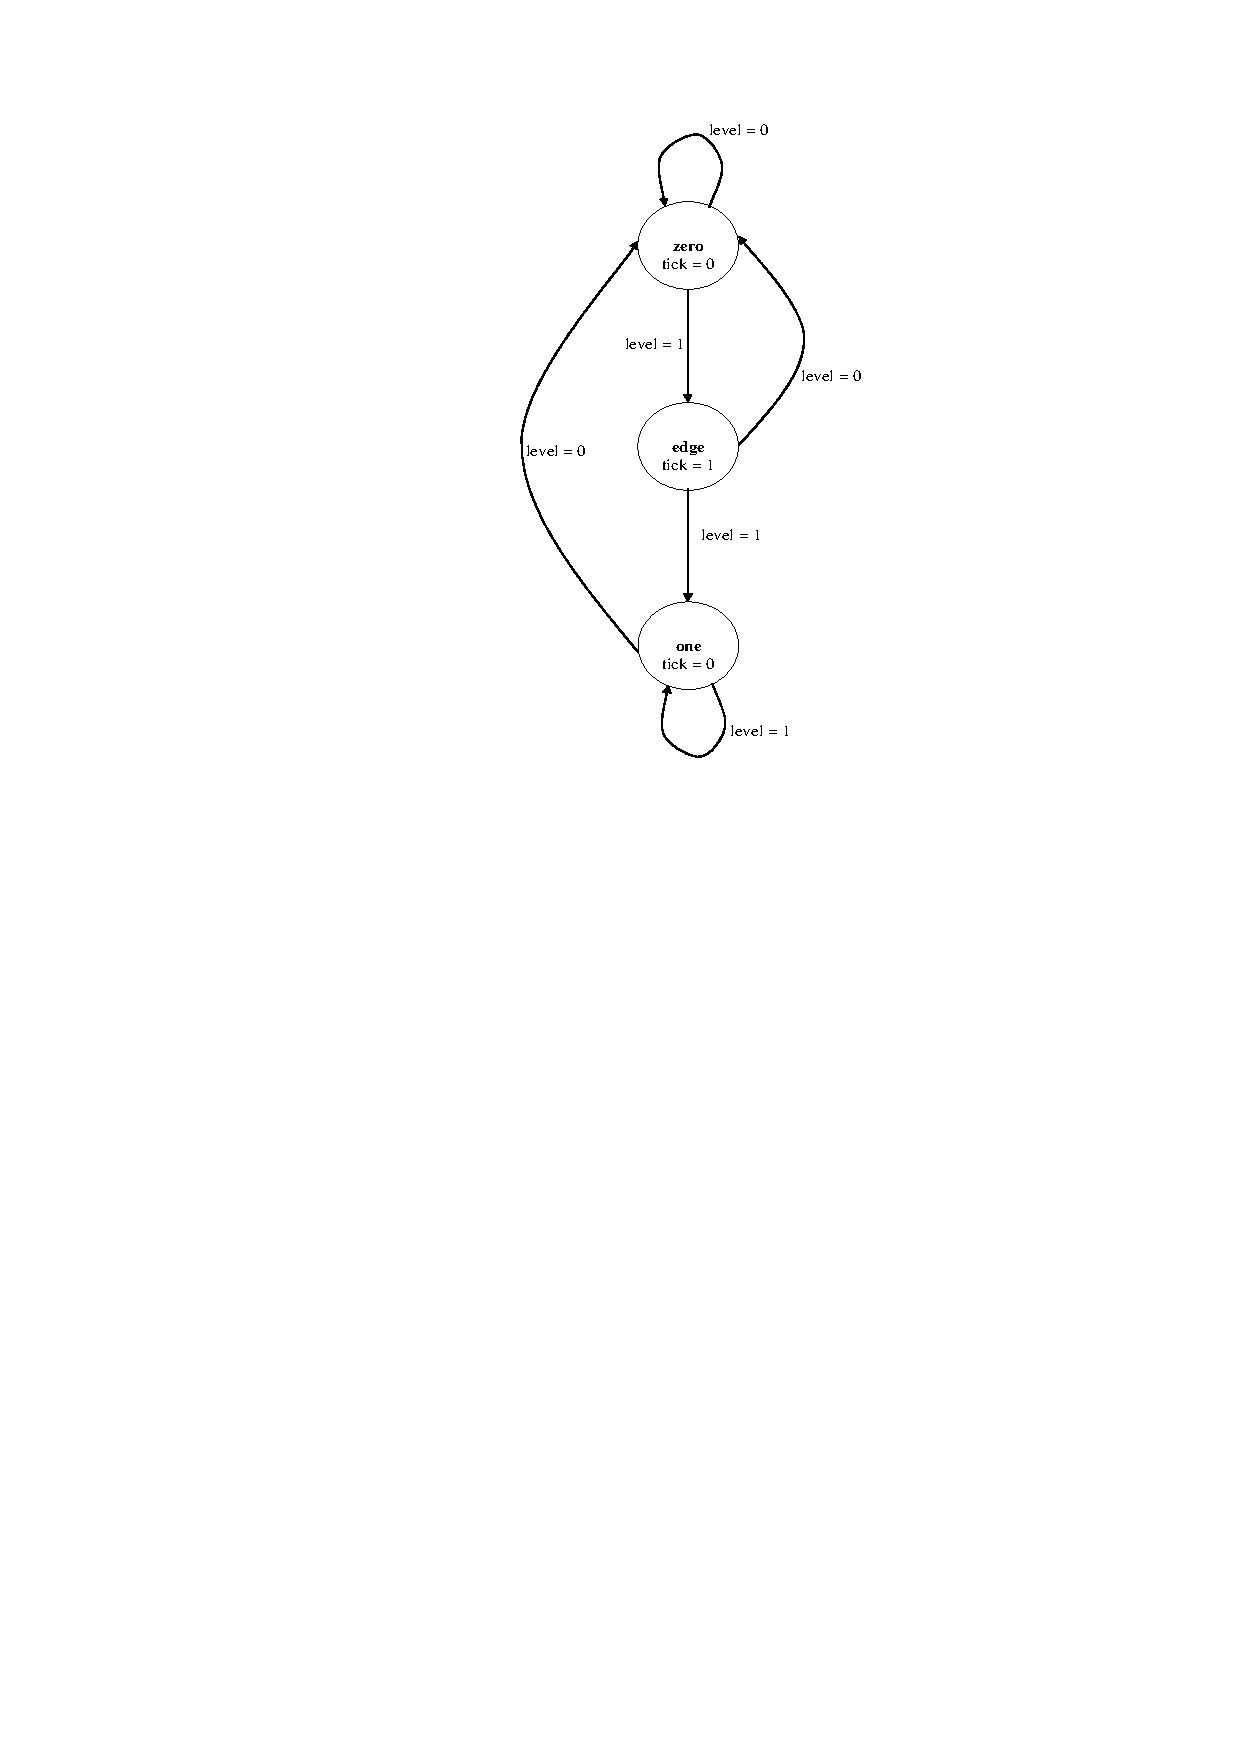
\includegraphics[scale=0.8]{MooreEdgeDetector}
		\caption{Moore Design}
		\label{fig:MooreEdgeDetector}
	\end{subfigure}
	\begin{subfigure}[!t]{0.45\textwidth}
		\centering
		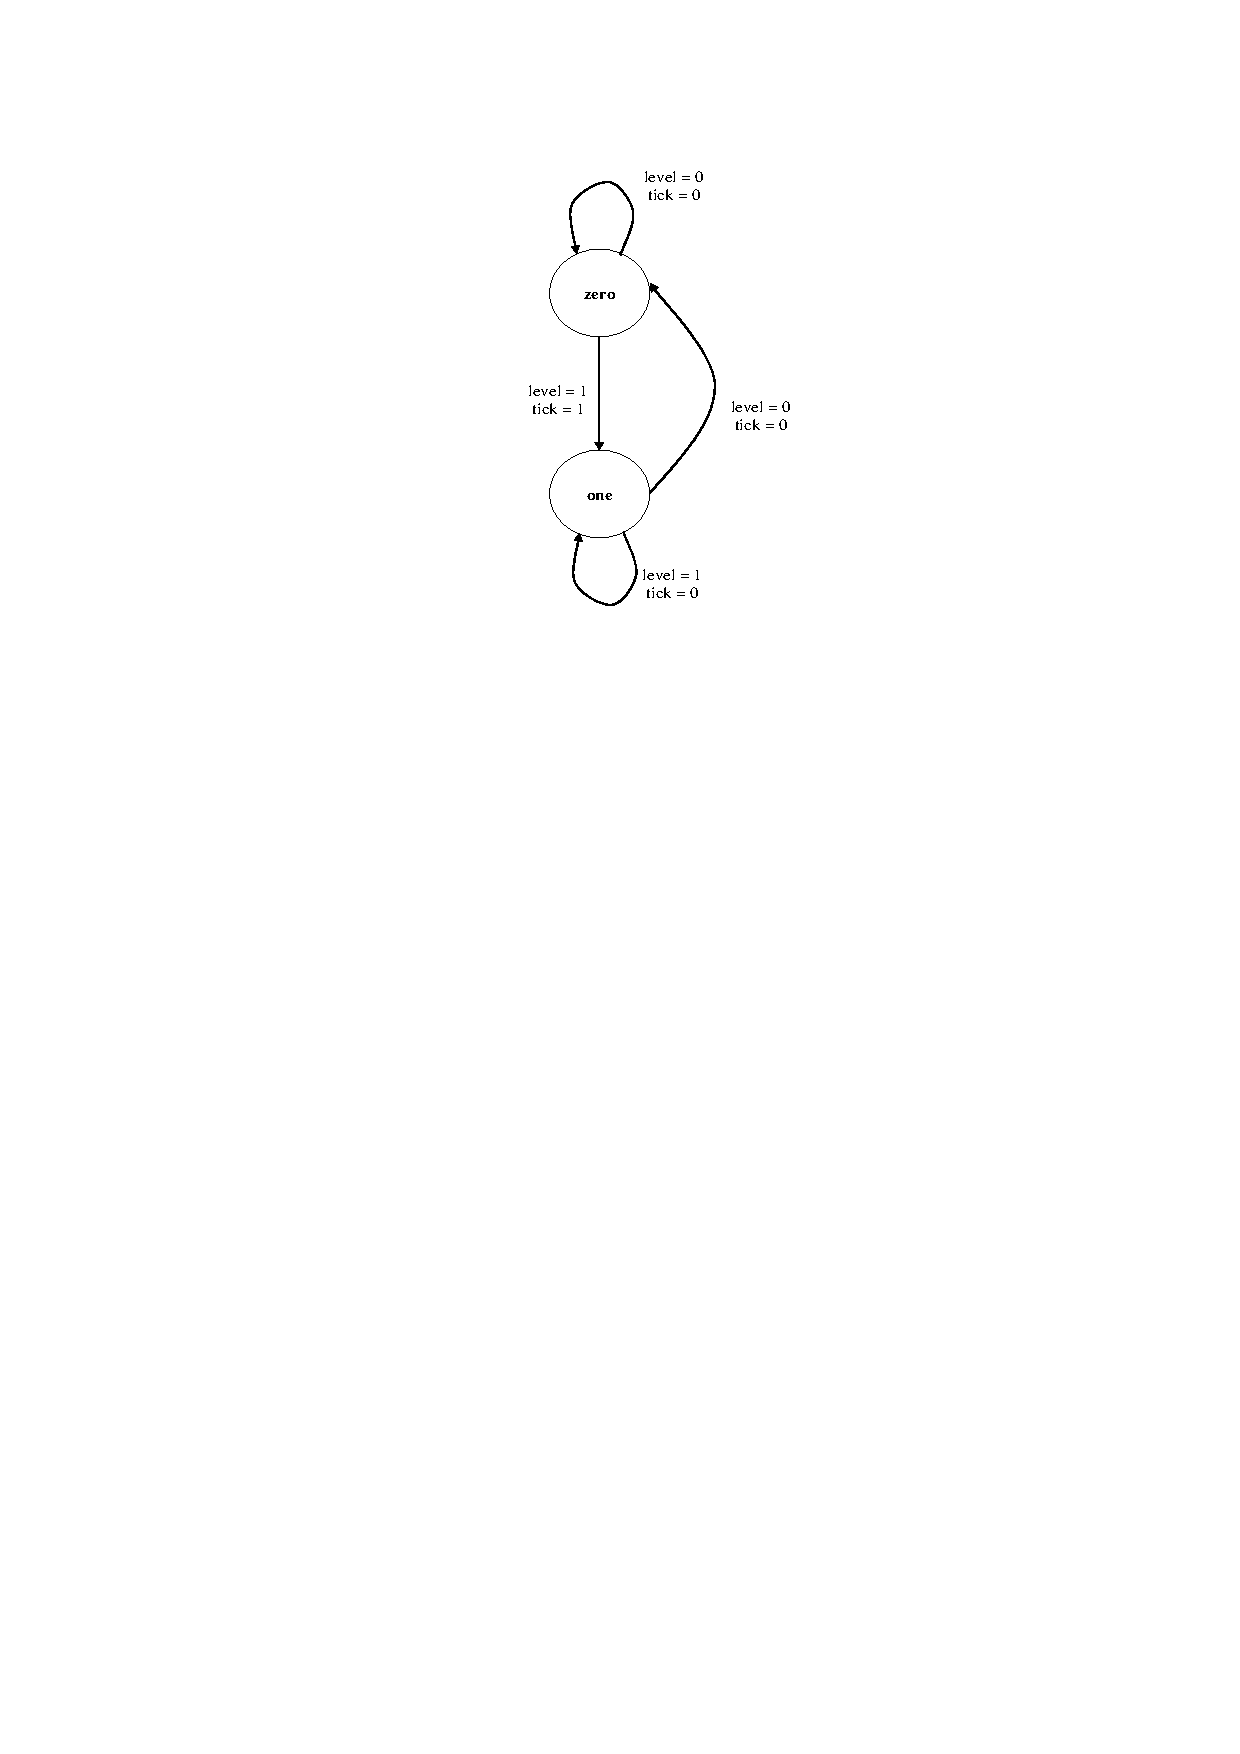
\includegraphics[scale=0.8]{MealyEdgeDetector}
		\caption{Mealy Design}
		\label{fig:MealyEdgeDetector}
	\end{subfigure}%	
	\caption{State diagrams for Edge detector }
	\label{fig:MealyMooreDect}
\end{figure}

\subsection{Implementation}
Both Mealy and Moore designs are implemented in Listing \ref{verilog:edgeDetector}. The listing can be seen as two parts i.e. Mealy design (Lines 37-55) and Moore design (Lines 57-80). Please read the comments for complete understanding of the code. The simulation waveforms i.e. Fig. \ref{fig:edgeDetectorWave} are discussed in next section. 
\lstinputlisting[
language = Verilog,
caption    = {Edge detector: Mealy and Moore designs},
label      = {verilog:edgeDetector}
]{edgeDetector.v}

\subsection{Outputs comparison}

In Fig. \ref{fig:edgeDetectorWave}, it can be seen that output-tick of Mealy detector is generated as soon as the `level' goes to 1, whereas Moore design generate the tick after 1 clock cycle. These two ticks are shown with the help of the two red cursors in the figure. Since, output of Mealy design is immediately available therefore it is preferred for synchronous designs. 

\begin{figure}[!h]
	\centering
	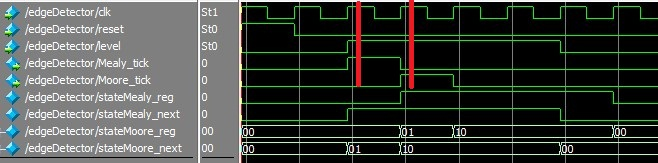
\includegraphics[width=\textwidth]{edgeDetectorWave}
	\caption{Simulation waveforms of rising edge detector in Listing \ref{verilog:edgeDetector}}
	\label{fig:edgeDetectorWave}
\end{figure}

\subsection{Visual verification}
Listing \ref{verilog:edgeDetector_VisualTest} can be used to verify the results on the FPGA board. Here, clock with 1 Hz frequency is used in line 19, which is defined in Listing \ref{verilog:clockTick}. After loading the design on FPGA board, we can observe on LEDs that the output of Moore design displayed after  Mealy design, with a delay of 1 second.  

\lstinputlisting[
language = Verilog,
caption    = {Visual verification of edge detector},
label      = {verilog:edgeDetector_VisualTest}
]{edgeDetector_VisualTest.v}



\section{Glitches} \label{sec:glitches}
Glitches are the short duration pulses which are generated in the combinational circuits. These are generated when more than two inputs change their values simultaneously. Glitches can be categorized as `static glitches' and `dynamic glitches'. Static glitches are further divided into two groups i.e. `static-0' and `static-1'. `Static-0' glitch is the glitch which occurs in logic `0' signal i.e. \textbf{one short pulse} i.e. `high-pulse (logic-1)' appears in logic-0 signal (and the signal settles down). Dynamic glitch is the glitch in which \textbf{multiple short pulses} appear before the signal settles down. 

\begin{noNumBox}
	Most of the times, the glitches are not the problem in the design. Glitches create problem when it occur in the outputs, which are used as clock for the other circuits. In this case, glitches will trigger the next circuits, which will result in incorrect outputs. In such cases, it is very important to remove these glitches. In this section, the glitches are shown for three cases. Since, clocks are used in synchronous designs, therefore Section \ref{sec:glitchInsSync} is of our main interest.
\end{noNumBox} 

\subsection{Combinational design in asynchronous circuit}
Table \ref{tbl:glitch_table} shows the truth-table for $2 \times 1$ multiplexer and corresponding Karnaugh map is shown in Fig. \ref{fig:glitch_sol}. Note that, the glitches occurs in the circuit, when we exclude the `red part' of the solution from the Fig. \ref{fig:glitch_sol}, which results in minimum-gate solution, but at the same time the solution is disjoint. To remove the glitch, we can add the prime-implicant in red-part as well. This solution is good, if there are few such gates are required; however if the number of inputs are very high, whose values are changing simultaneously then this solution is not practical, as we need to add large number of gates.

\begin{table}[!h]
	\centering
	\caption{Truth table of $2 \times 1$ Multiplexer}
	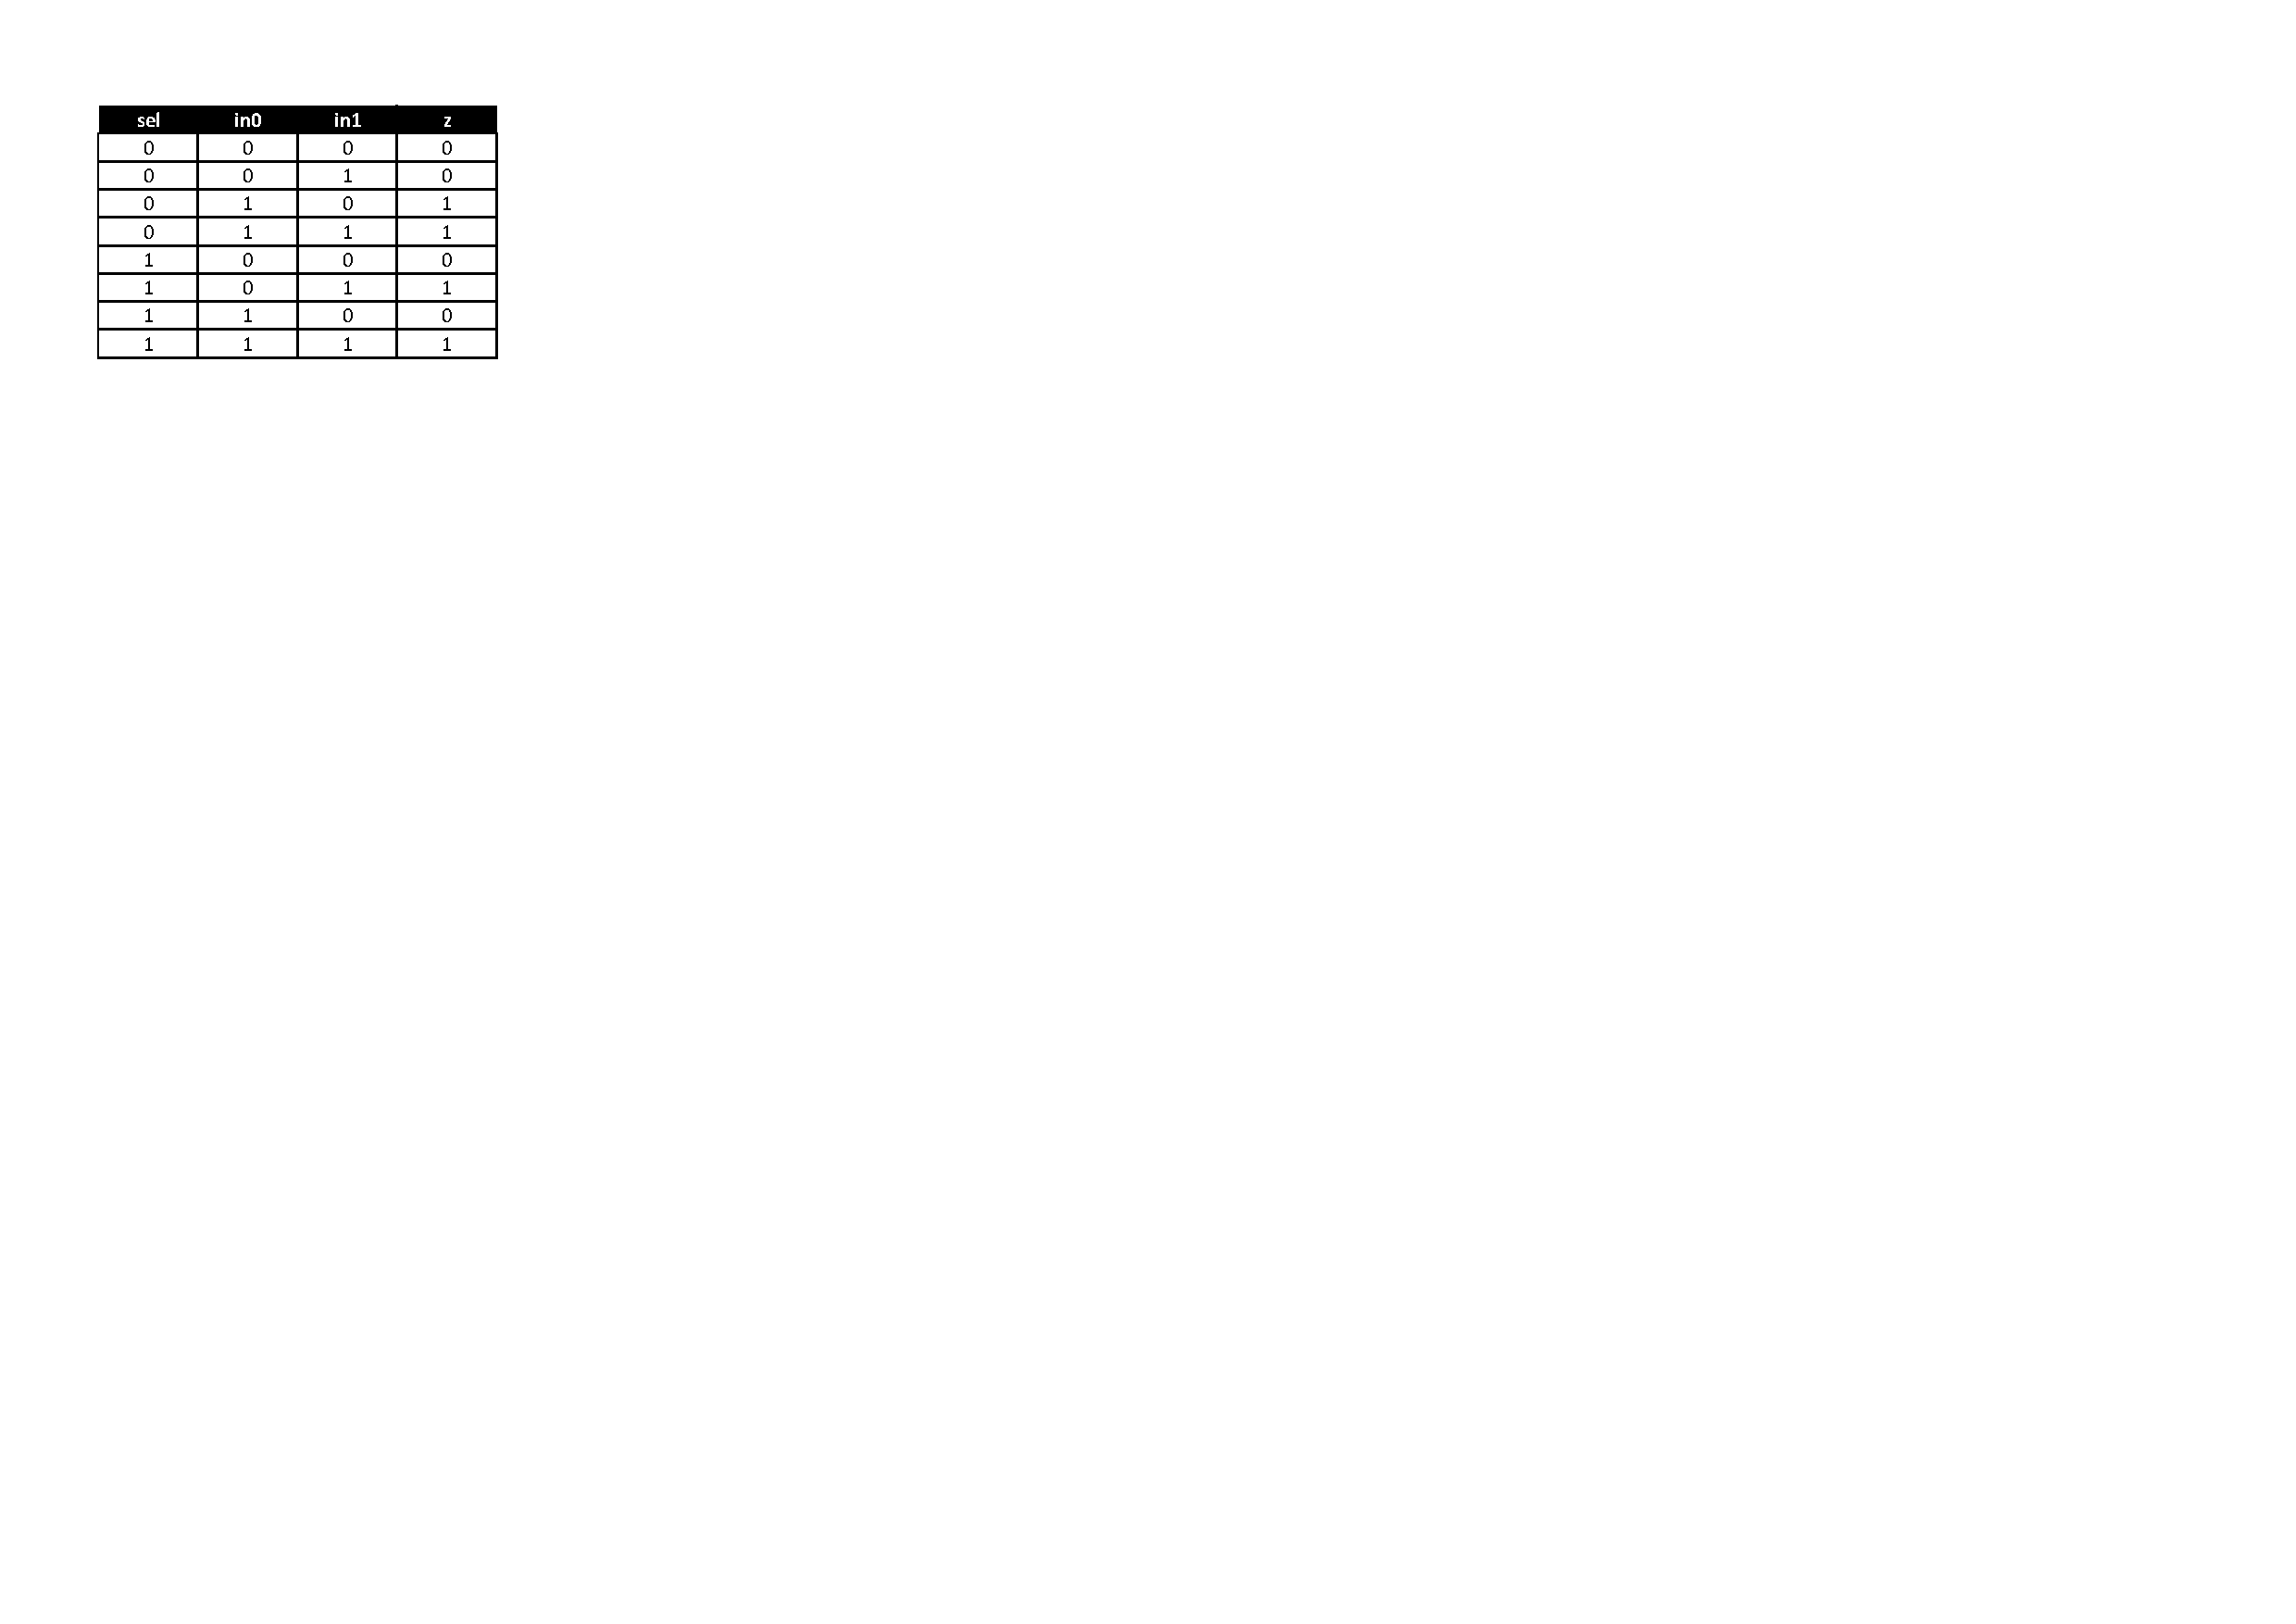
\includegraphics[scale = 1]{glitch_table}
	\label{tbl:glitch_table}
\end{table}

\begin{figure}[!h]
	\centering
	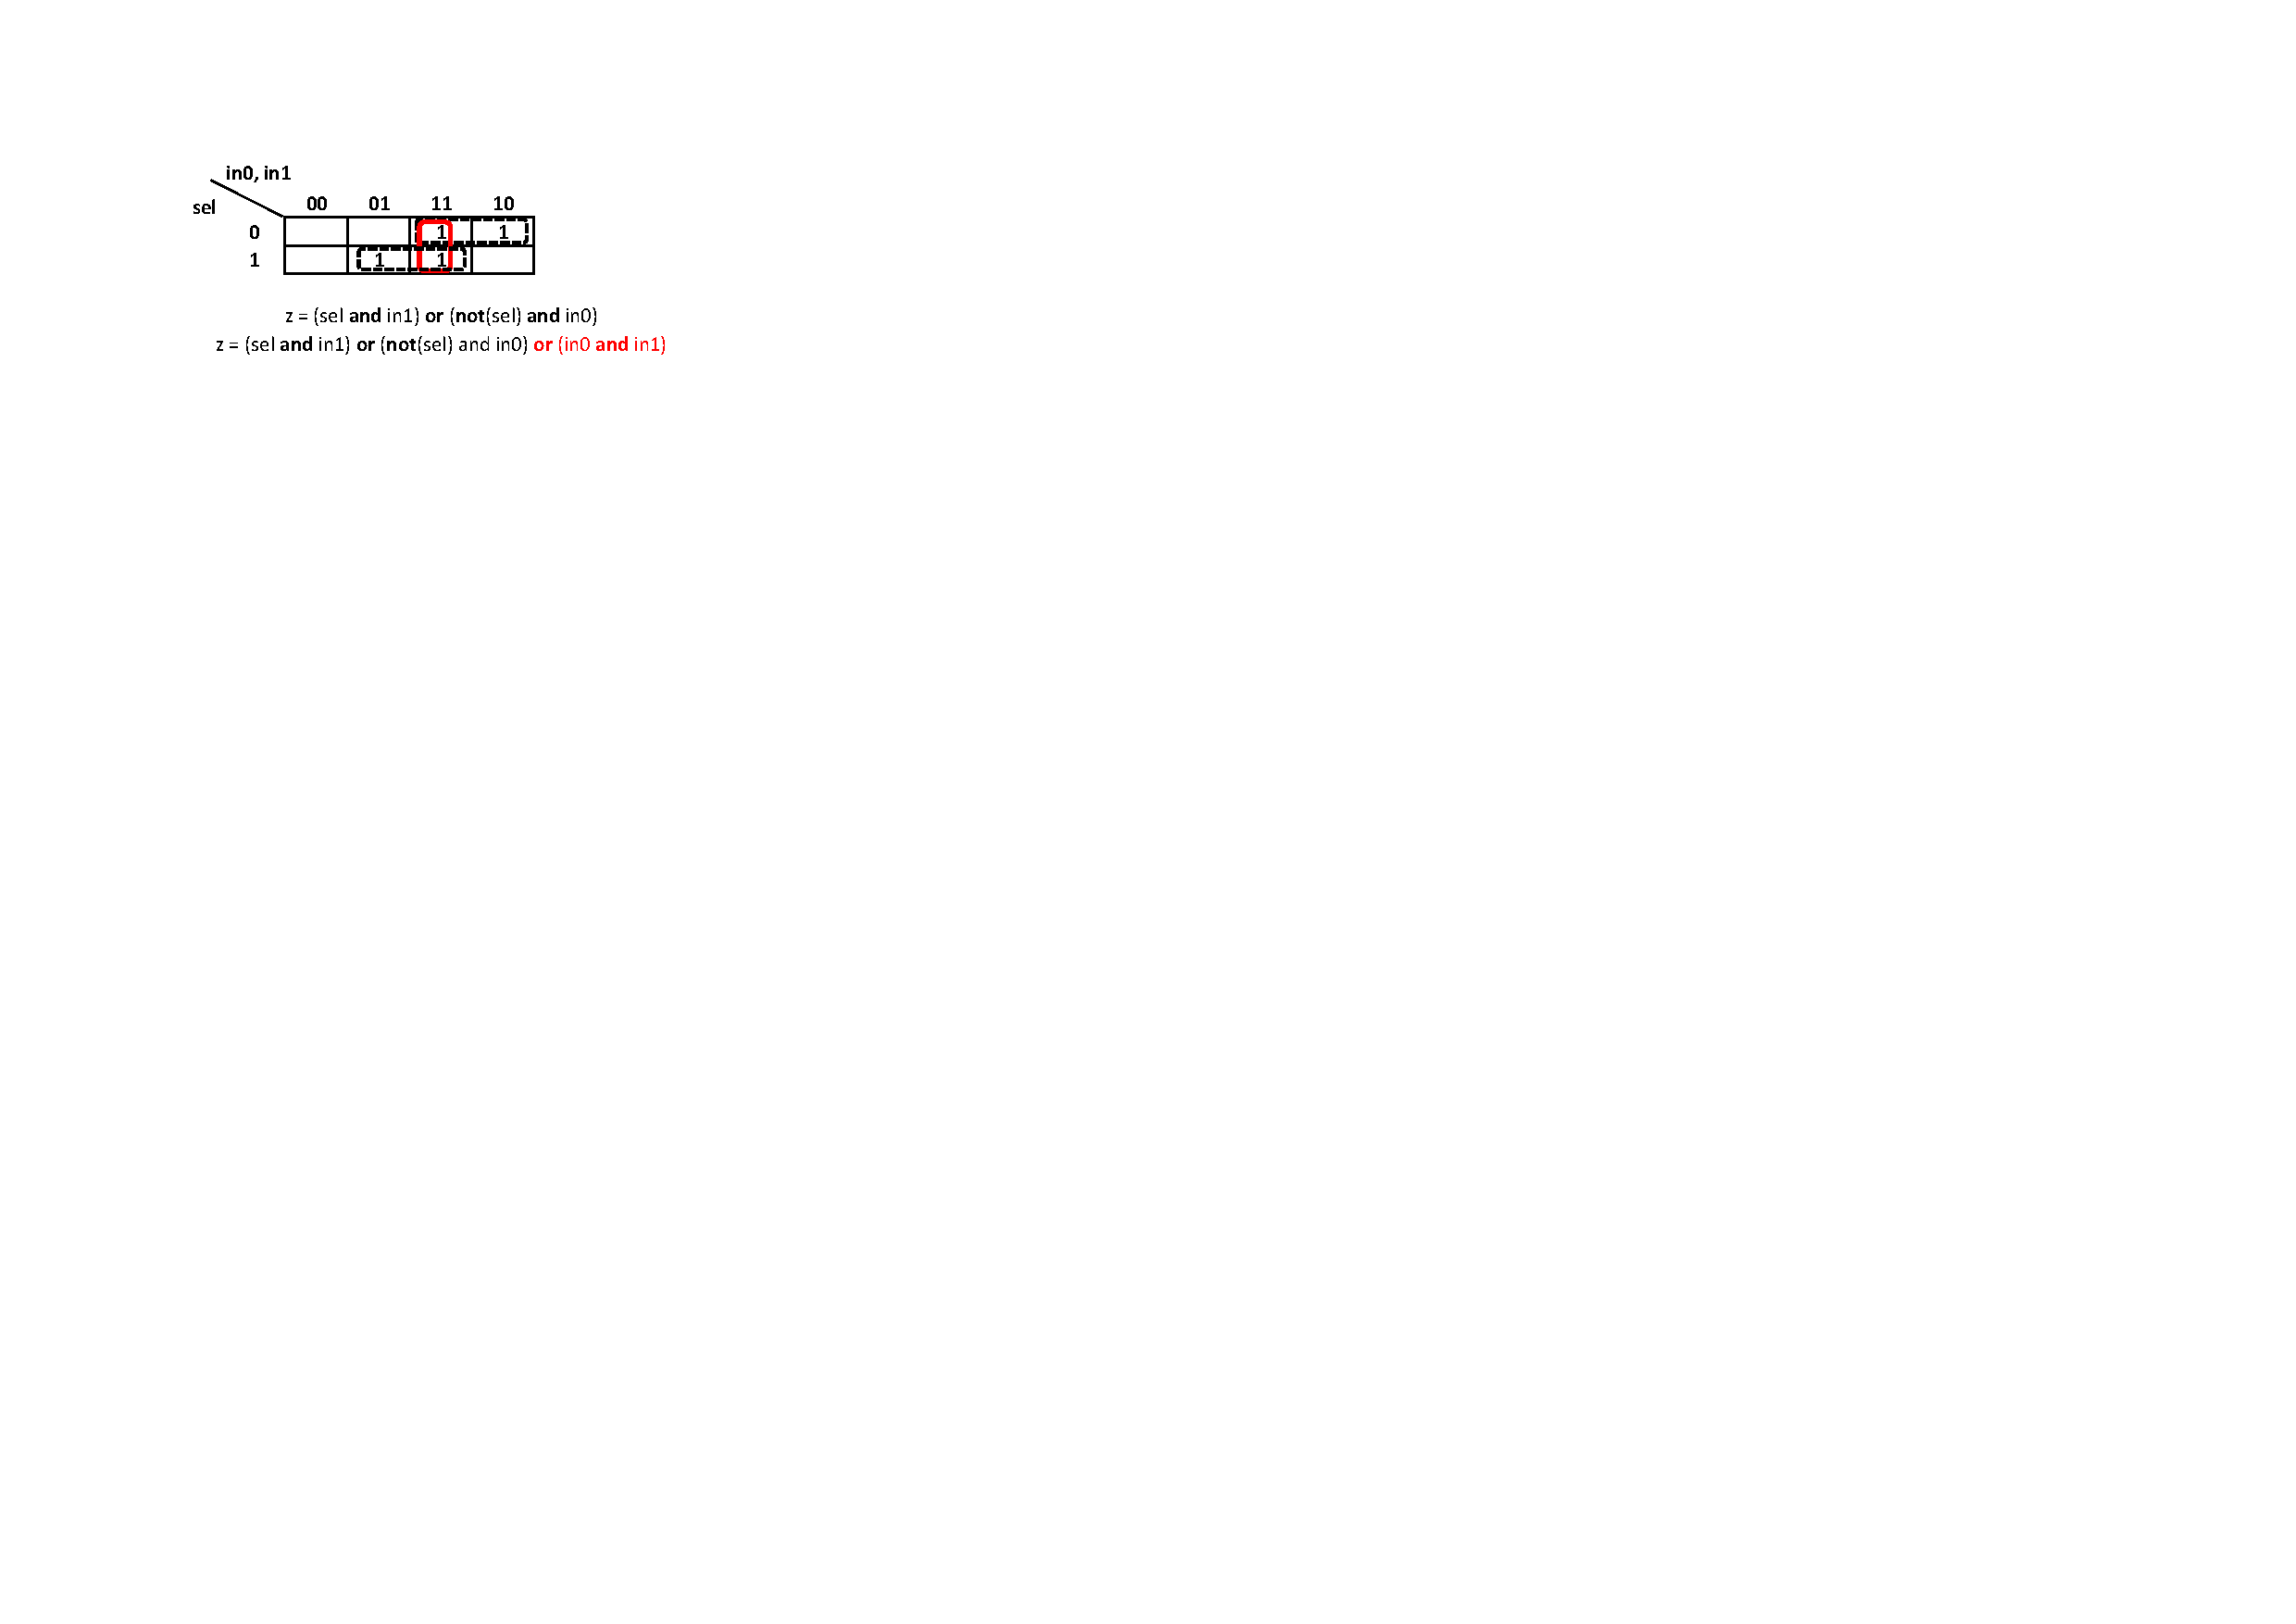
\includegraphics[scale = 1]{glitch_sol}
	\caption{Reason for glitches and solution}
	\label{fig:glitch_sol}
\end{figure}

\begin{figure}[!h]
	\centering
	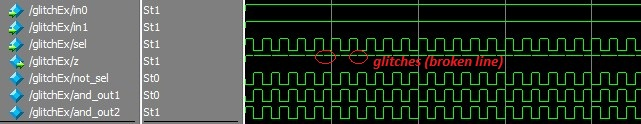
\includegraphics[width=\textwidth]{glitches}
	\caption{Glitches (see disjoint lines in `z') in design in Listing \ref{verilog:glitchEx}}
	\label{fig:glitches}
\end{figure}

\lstinputlisting[
language = Verilog,
caption    = {Glitches in multiplexer},
label      = {verilog:glitchEx}
]{glitchEx.v}

\subsection{Unfixable Glitch}
Listing \ref{verilog:manchester_code} is another example of glitches in the design as shown in Fig. \ref{fig:manchesterGlitch}. Here, glitches are continuous i.e. these are occurring at every change in signal `din'. Such glitches are removed by using D-flip-flop as shown in Section \ref{sec:glitchInsSync}. \textbf{Since the output of Manchester code depends on both edges of clock (i.e. half of the output changes on $+ve$ edge and other half changes at $-ve$ edge), therefore such glitches are unfixable; as in Verilog both edges can not be connected to one D flip flop.}

\begin{figure}[!h]
	\centering
	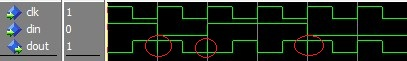
\includegraphics[width=\textwidth]{manchesterGlitch}
	\caption{Glitches in Listing \ref{verilog:manchester_code}}
	\label{fig:manchesterGlitch}
\end{figure}

\lstinputlisting[
language = Verilog,
caption    = {Glitches in Manchester coding},
label      = {verilog:manchester_code}
]{manchester_code.v}


\subsection{Combinational design in synchronous circuit}\label{sec:glitchInsSync}
Combination designs in sequential circuits were discussed in Fig. \ref{fig:combSeqBlock}. The output of these combination designs can depend on states only, or on the states along with external inputs. The former is known as Moore design and latter is known as Mealy design as discussed in Section \ref{sec:MealyMooreDesign}. Since, the sequential designs are sensitive to edge of the clock, therefore the glitches can occur only at the edge of the clock. Hence, the glitches at the edge can be removed by sending the output signal through the D flip flop, as shown in Fig. \ref{fig:combSeqBlockGlitchFree}. Various Verilog templates for sequential designs are shown in Section \ref{sec:MooreTemplates} and \ref{sec:MealyTemplates}. 

\begin{figure}[!h]
	\centering
	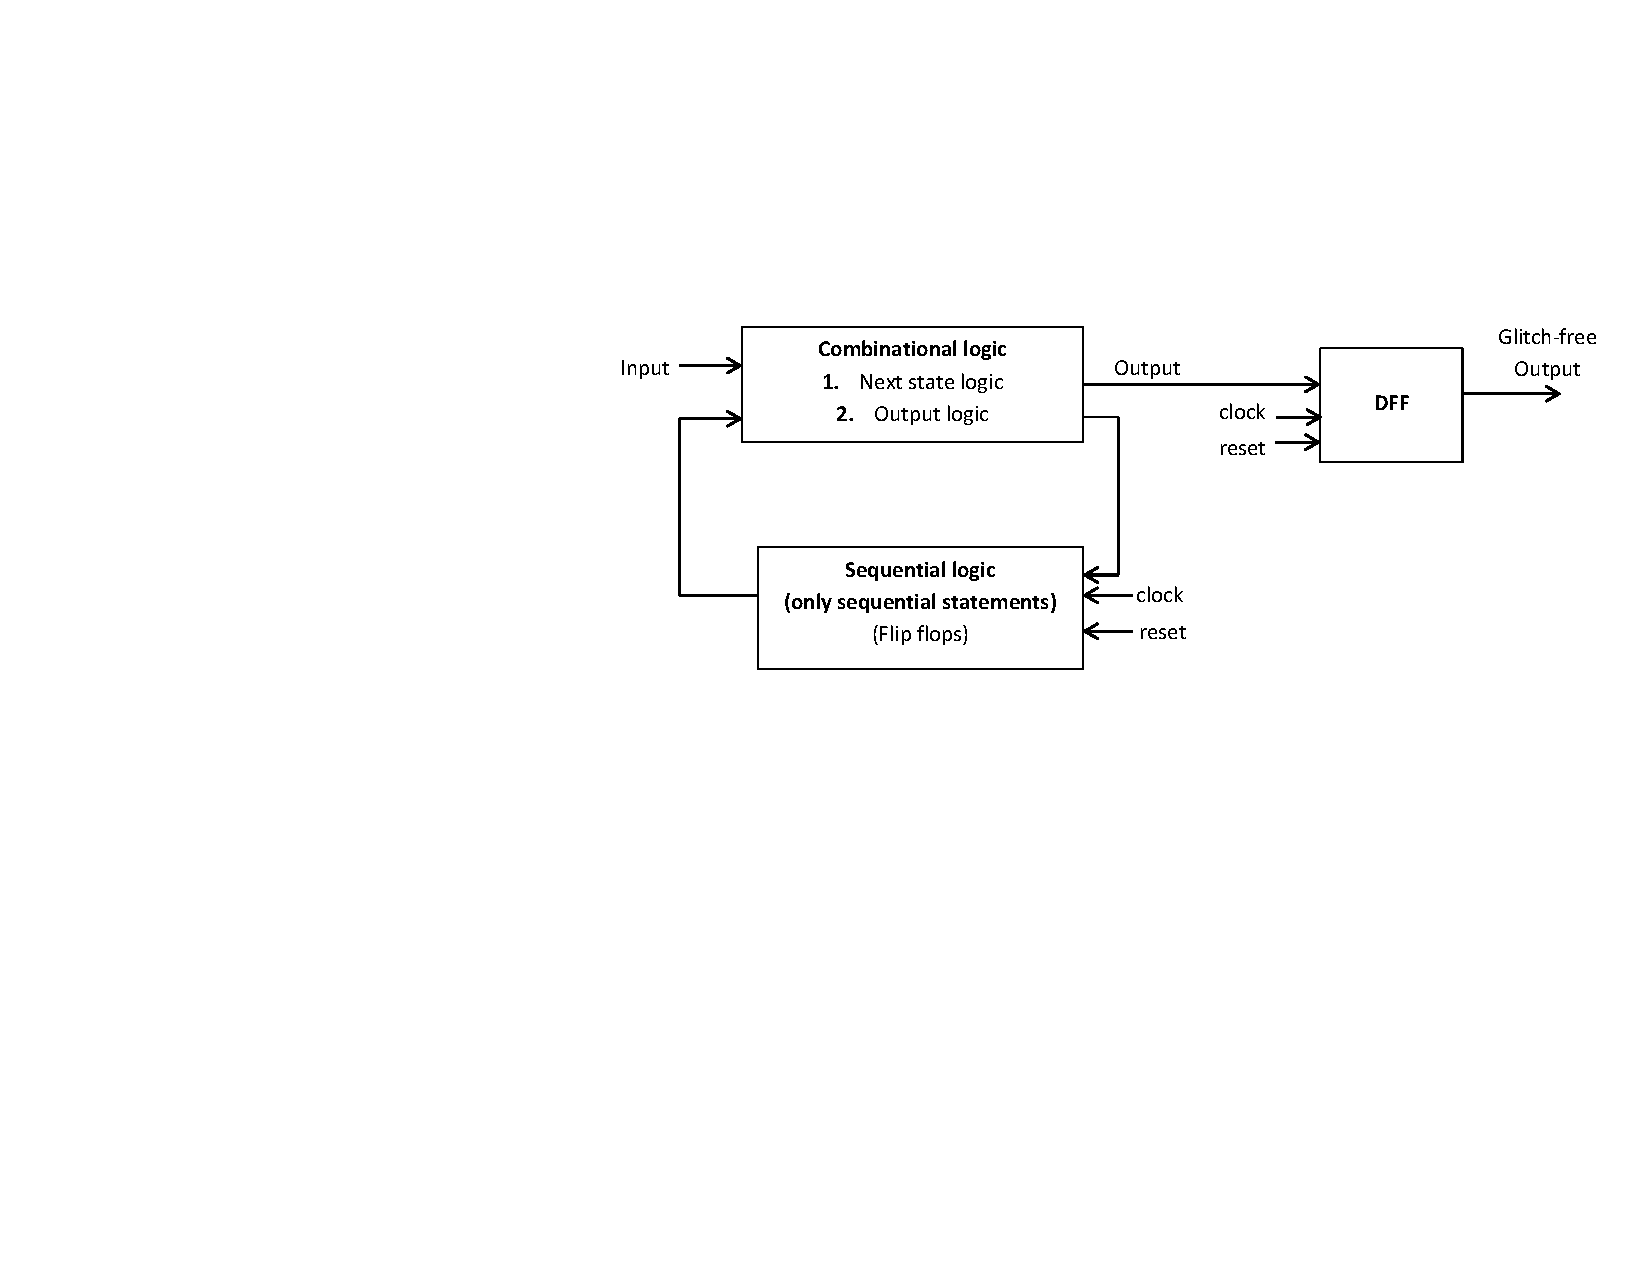
\includegraphics[scale = 0.8]{combSeqBlockGlitchFree}
	\caption{Glitch-free sequential design using D flip flop}
	\label{fig:combSeqBlockGlitchFree}
\end{figure}


\section{Moore architecture and Verilog templates} \label{sec:MooreTemplates}
Fig. \ref{fig:combSeqBlockGlitchFree} shows the different block for the sequential design. In this figure, we have three blocks i.e. `sequential logic', `combinational logic' and `glitch removal block'. In this section, we will define three process-statements to implemented these blocks (see Listing \ref{verilog:moore_regular_template2}). Further, `combinational logic block' contains two different logics i.e. `next-state' and `output'. Therefore, this block can be implemented using two different block, which will result in four process-statements (see Listing \ref{verilog:moore_regular_template}). 

Moore and Mealy machines can be divided into three categories i.e. `regular', 'timed' and `recursive'. The differences in these categories are shown in Fig. \ref{fig:typeMooreMachine} for Moore machine. In this section, we will see different Verilog templates for these categories. Note that, the design may be the combinations of these three categories, and we need to select the correct template according to the need. Further, the examples of these templates are shown in Section \ref{sec:VerilogtemplateExample}.


\begin{figure*}[!h]
	\begin{subfigure}[t]{1\textwidth}
		\centering
		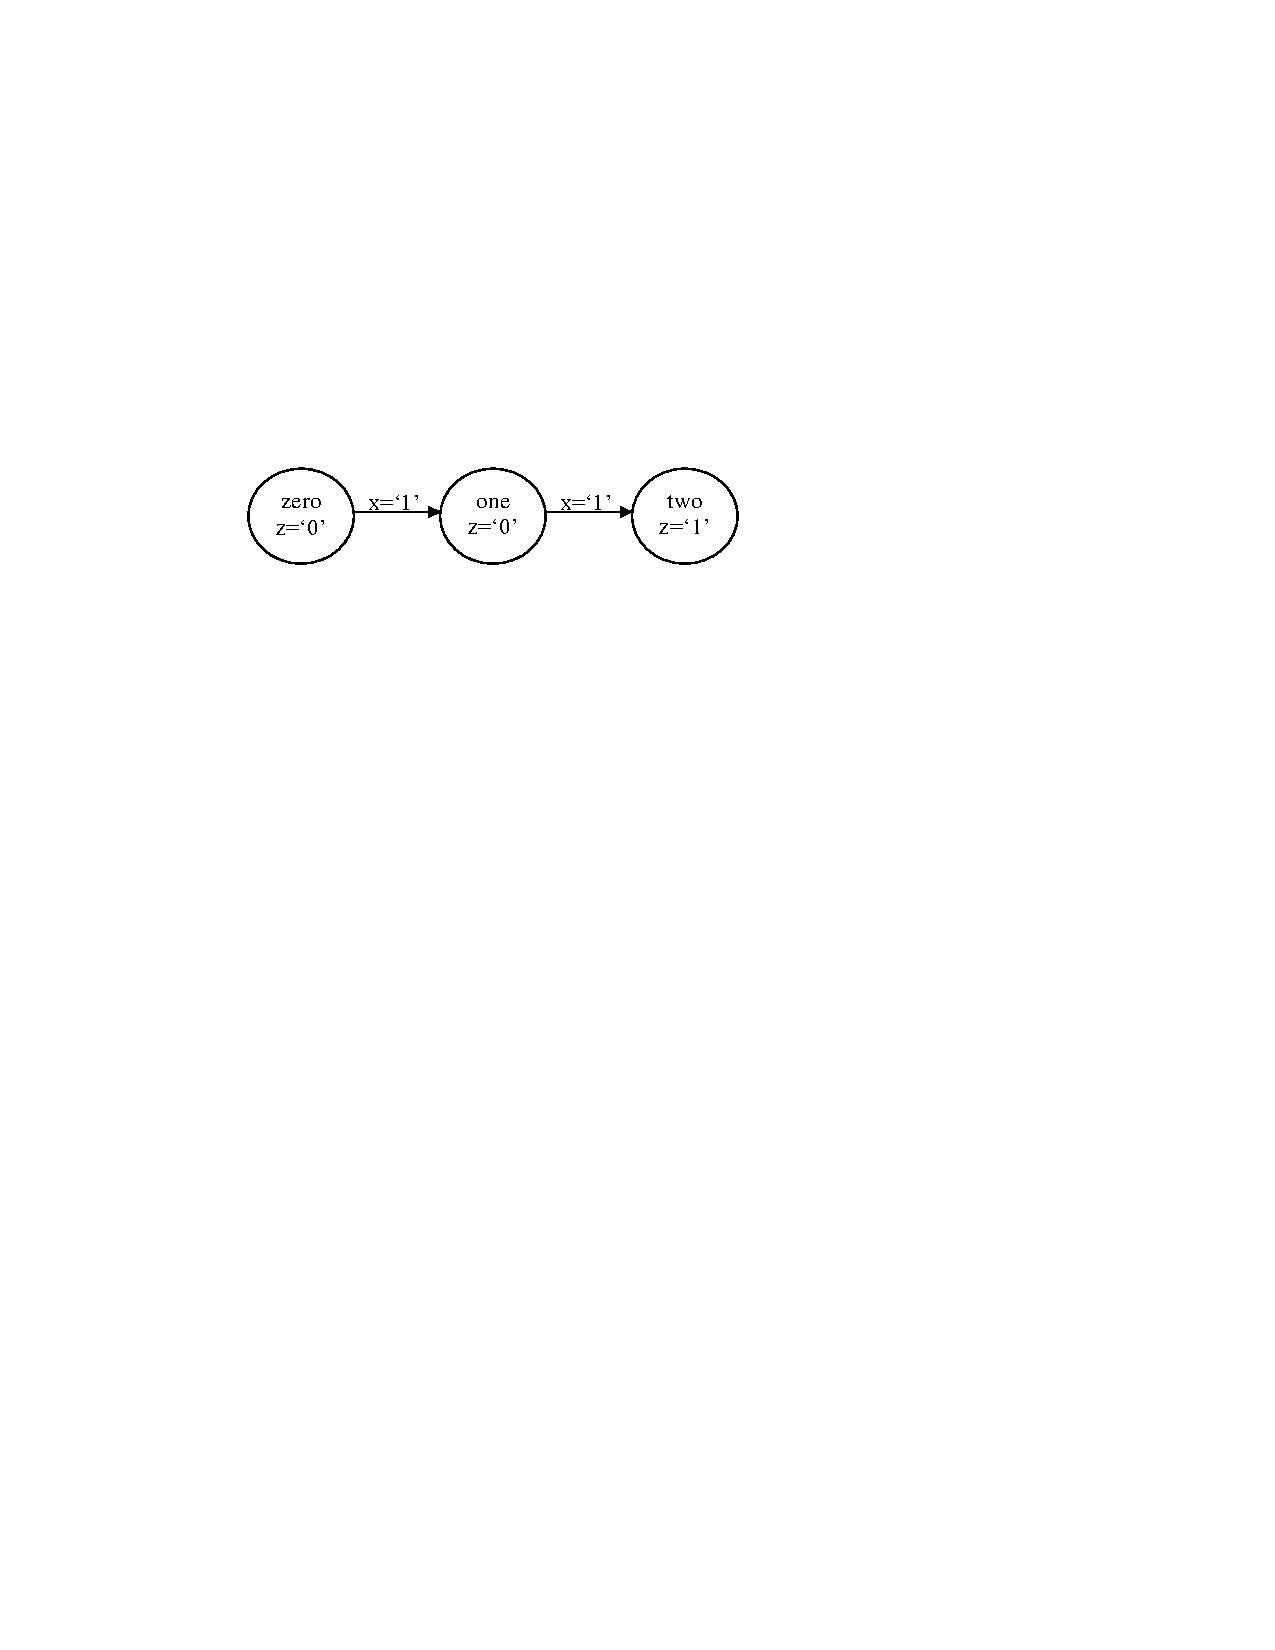
\includegraphics[width=0.5\columnwidth]{regular}
		\caption{Regular Moore machine}
		\label{subfig:regular}
	\end{subfigure} %  
	\begin{subfigure}[t]{1\textwidth}
		\centering
		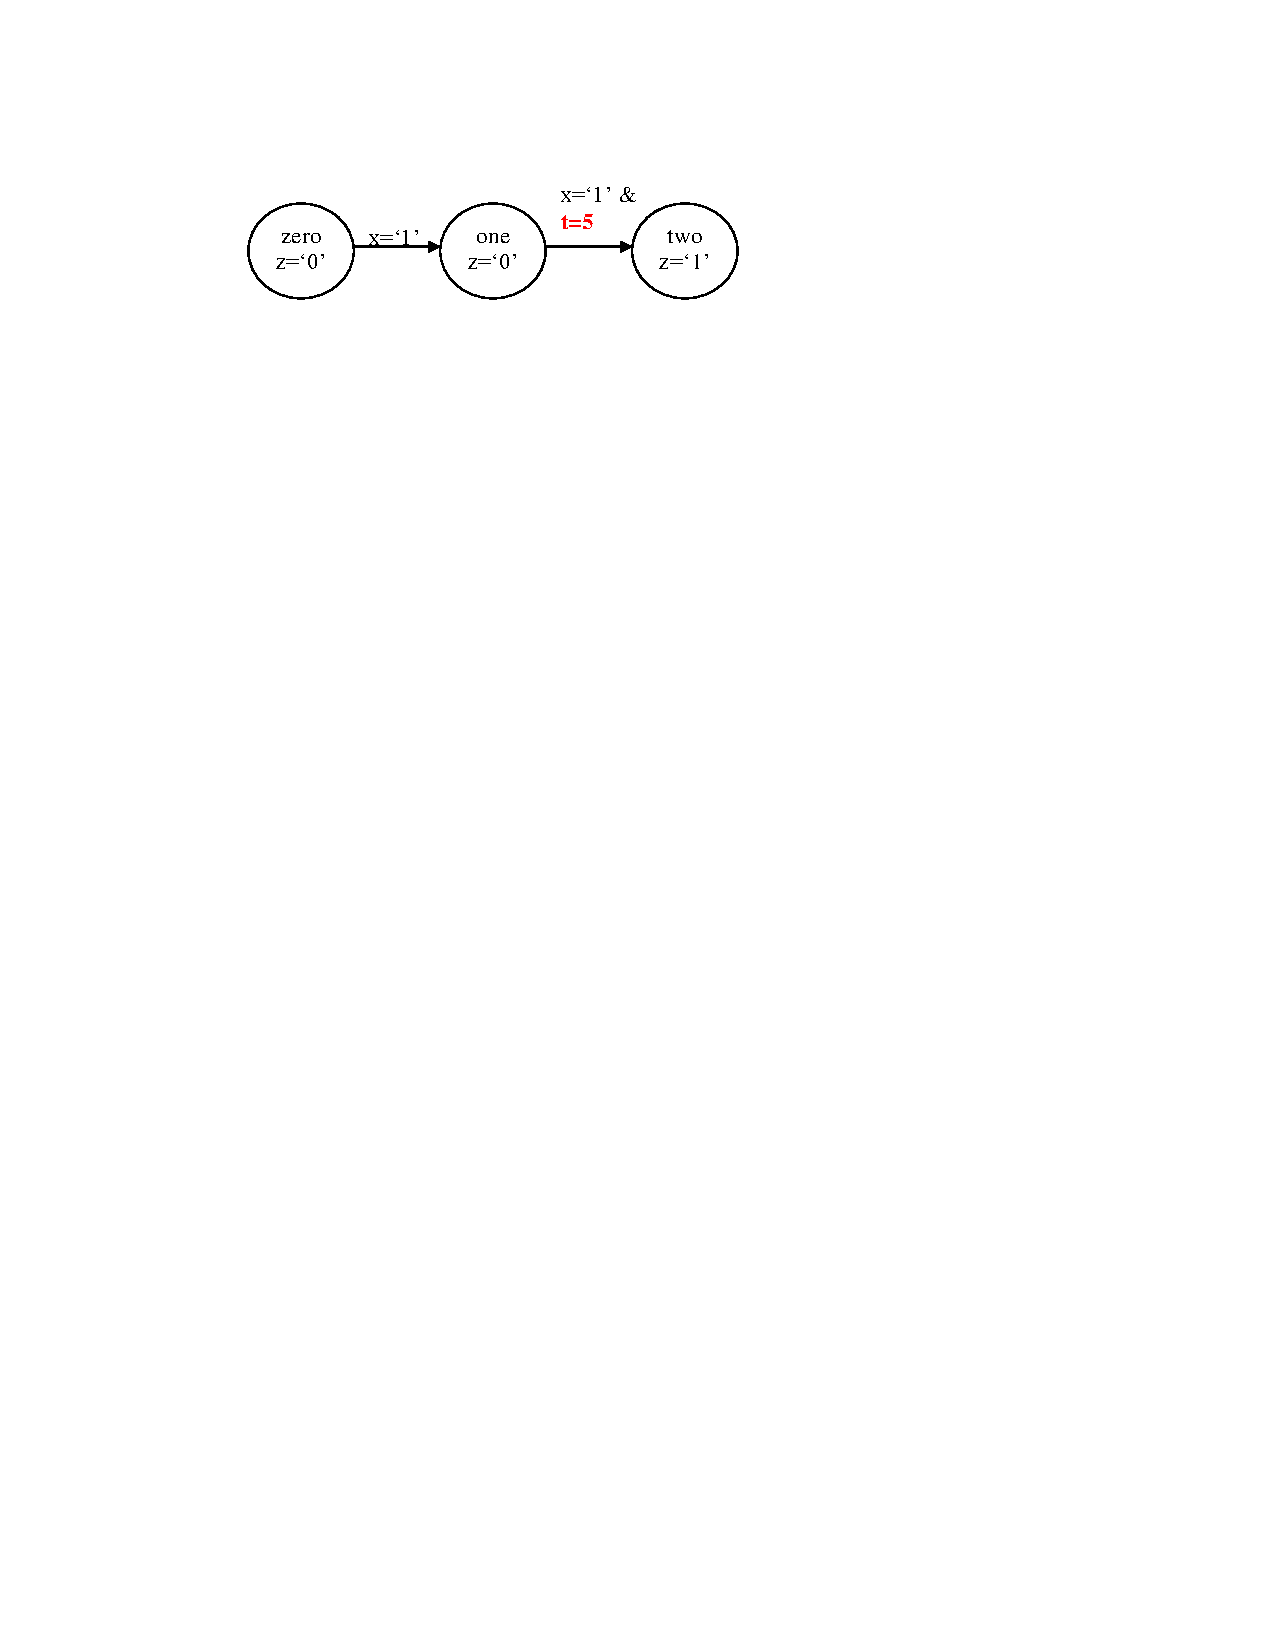
\includegraphics[width=0.5\columnwidth]{timed}
		\caption{Timed Moore machine : next state depends on time as well}
		\label{subfig:timed}
	\end{subfigure}	
	
	\begin{subfigure}[t]{1\textwidth}
		\centering
		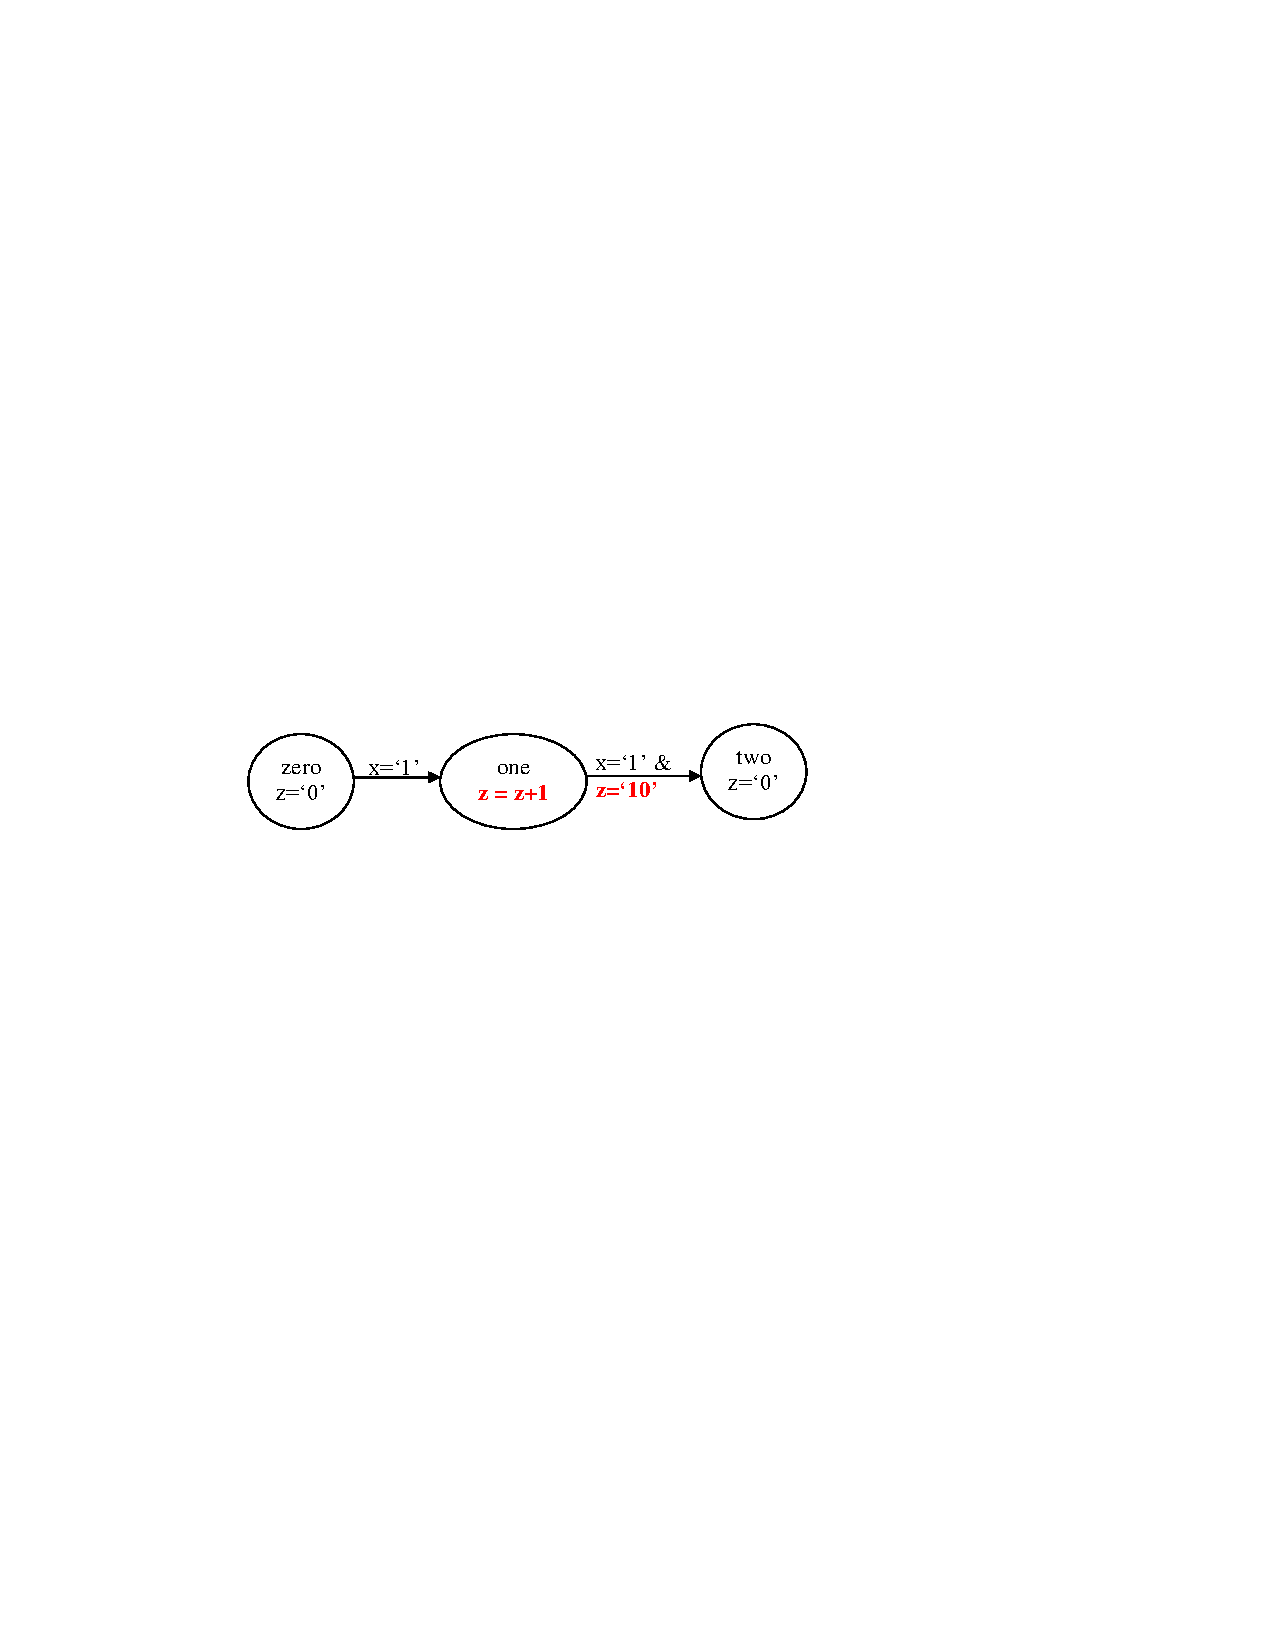
\includegraphics[width=0.5\columnwidth]{recursive}
		\caption{Recursive Moore machine : output `z' depends on output i.e. feedback required}
		\label{subfig:recursive}
	\end{subfigure}	
	\caption{Different types of FSM}
	\label{fig:typeMooreMachine}%
\end{figure*}


\subsection{Regular machine}
Please see the Fig. \ref{subfig:regular} and note the following points about regular Moore machine, 
\begin{enumerate}
	\item Output depends only on the states, therefore \textbf{no `if statement'} is required in the process-statement. For example, in Lines 85-87 of Listing \ref{verilog:moore_regular_template}, the outputs (Lines 86-87) are defined inside the `s0' (Line 86). 
	\item Next-state depends on current-state and and  \textbf{current external inputs}. For example, the `state\_next' at Line 49 of Listing \ref{verilog:moore_regular_template} is defined inside `if statement' (Line 48) which depends on current input. Further, this `if statement' is defined inside the state `s0' (Line 47). Hence the next state depends on current state and current external input.    
\end{enumerate}

\begin{noNumBox}
	In regular Moore machine, 
	\begin{enumerate}
		\item Outputs depend on current external inputs. 
		\item Next states depend on current states and current external inputs.
	\end{enumerate}
\end{noNumBox}

\lstinputlisting[
language = Verilog,
caption    = {Verilog template for regular Moore FSM : separate `next\_state' and `output' logic},
label      = {verilog:moore_regular_template}
]{moore_regular_template.v}

Listing \ref{verilog:moore_regular_template2} is same as Listing \ref{verilog:moore_regular_template}, but the ouput-logic and next-state logic are combined in one process block. 

\lstinputlisting[
language = Verilog,
caption    = {Verilog template for regular Moore FSM : combined `next\_state' and `output' logic},
label      = {verilog:moore_regular_template2}
]{moore_regular_template2.v}


\subsection{Timed machine}
If the state of the design changes after certain duration (see Fig. \ref{subfig:timed}), then we need to add the timer in the Verilog design which are created in Listing \ref{verilog:moore_regular_template} and \ref{verilog:moore_regular_template}. For this, we need to add one more process-block which performs following actions, 
\begin{itemize}
	\item \textbf{Zero the timer : } The value of the timer is set to zero, whenever the state of the system changes. 
	\item \textbf{Stop the timer : } Value of the timer is incremented till the predefined `maximum value' is reached and then it should be stopped incrementing. Further, it's value should \textbf{not} be set to zero until state is changed. 
\end{itemize}

\begin{noNumBox}
	In timed Moore machine, 
	\begin{enumerate}
		\item Outputs depend on current external inputs. 
		\item Next states depend on time along with current states and current external inputs.
	\end{enumerate}
\end{noNumBox}
Template for timed Moore machine is shown in Listing \ref{verilog:moore_timed_template}, which is exactly same as Listing \ref{verilog:moore_regular_template2} except with following changes, 
\begin{enumerate}
	\item Timer related constants are added at Line 22-27.
	\item An `always' block is added to stop and zero the timer (Lines 44-54). 
	\item Finally, timer related conditions are included for next-state logic e.g.  Lines 64 and 67 etc.
\end{enumerate}

\lstinputlisting[
language = Verilog,
caption    = {Verilog template timed Moore FSM : separate `next\_state' and `output' logic},
label      = {verilog:moore_timed_template}
]{moore_timed_template.v}

\subsection{Recursive machine}
In recursive machine, the outputs are fed back as input to the system (see Fig. \ref{subfig:recursive}). Hence, we need additional process-statement which can store the outputs which are fed back to combinational block of sequential design, as shown in Listing \ref{verilog:moore_recursive_template}. The listing is same as Listing \ref{verilog:moore_timed_template} except certain signals and process block are defined to feedback the output to combination logic; i.e. Lines 29-31 contain the signals (feedback registers) which are required to be feedback the outputs. Here, `\_next' and `\_reg' are used in these lines, where `next' value is fed back as `reg' in the next clock cycle inside the `always' statement which is defined in Lines 63-75. Lastly, `feedback registers' are also used to calculate the next-state inside the `if statement' e.g. Lines 91 and 96. Also, the value of feedback registers are updated inside these `if statements' e.g. Lines 93 and 102. 

\begin{noNumBox}
	In recursive Moore machine, 
	\begin{enumerate}
		\item Outputs depend on current external inputs. Also, values in the feedback registers are used as outputs.
		\item Next states depend current states, current external input, current internal inputs (i.e. previous outputs feedback as inputs to system) and time (optional).
	\end{enumerate}
\end{noNumBox}

\lstinputlisting[
language = Verilog,
caption    = {Verilog template recursive Moore FSM : separate `next\_state' and `output' logic},
label      = {verilog:moore_recursive_template}
]{moore_recursive_template.v}


\section{Mealy architecture and Verilog templates} \label{sec:MealyTemplates}
Template for Mealy architecture is similar to Moore architecture. The minor changes are required as outputs depend on current input as well, as discussed in this section.
\subsection{Regular machine}
In Mealy machines, the output is the function of current input and states, therefore the output will also defined inside the if-statements (Lines 49-50 etc.). Rest of the code is same as Listing \ref{verilog:moore_regular_template2}. 
\lstinputlisting[
language = Verilog,
caption    = {Verilog template for regular Mealy FSM : combined `next\_state' and `output' logic},
label      = {verilog:mealy_regular_template}
]{mealy_regular_template.v}


\subsection{Timed machine}
Listing \ref{verilog:mealy_timed_template} contains timer related changes in Listing \ref{verilog:mealy_regular_template}. See description of Listing \ref{verilog:moore_timed_template} for more details. 
\lstinputlisting[
language = Verilog,
caption    = {Verilog template for timed Mealy FSM : combined `next\_state' and `output' logic},
label      = {verilog:mealy_timed_template}
]{mealy_timed_template.v}

\subsection{Recursive machine}

Listing \ref{verilog:mealy_recursive_template} contains recursive-design related changes in Listing \ref{verilog:mealy_timed_template}. See description of Listing \ref{verilog:moore_recursive_template} for more details. 

\lstinputlisting[
language = Verilog,
caption    = {Verilog template for recursive Mealy FSM : combined `next\_state' and `output' logic},
label      = {verilog:mealy_recursive_template}
]{mealy_recursive_template.v}


\section{Examples} \label{sec:VerilogtemplateExample}

\subsection{Regular Machine : Glitch-free Mealy and Moore design} \label{sec:exampleRegularMMGlitchFree}
In this section, a non-overlapping sequence detector is implemented to show the differences between Mealy and Moore machines. Listing \ref{verilog:sequence_detector} implements the `sequence detector' which detects the sequence `110'; and corresponding state-diagrams are shown in Fig. \ref{fig:non-overlap-design}. The RTL view generated by the listing is shown in Fig. \ref{fig:Mealy_Moore_RTL_glitchfree}, where two D-FF are added to remove the glitches from Moore and Mealy model. Also, in the figure, if we click on the state machines, then we can see the implemented state-diagrams e.g. if we click on `state\_reg\_mealy' then the state-diagram in Fig. \ref{fig:Altera_Mealy_seq_det_state} will be displayed, which is exactly same as Fig. \ref{subfig:Mealy_seq_det_state}. 


Further, the testbench for the listing is shown in Listing \ref{verilog:sequence_detector_tb}, whose results are illustrated in Fig. \ref{fig:Mealy_MooreGlitchFree}. Please note the following points in Fig. \ref{fig:Mealy_MooreGlitchFree},
\begin{enumerate}
	\item Mealy machines are asynchronous as the output changes as soon as the input changes. It does not wait for the next cycle. 
	\item If the output of the Mealy machine is delayed, then glitch will be removed and the output will be same as the Moore output\footnote{Note that, there is no glitch in this system. This example shows how to implement the D-FF to remove glitch in the system (if exists)}. 
	\item Glitch-free Moore output is delayed by one clock cycle. 
	\item If glitch is not a problem, then we should use Moore machine, because it is synchronous in nature. But, if glitch is problem and we do not want to delay the output then Mealy machines should be used. 
\end{enumerate}

\begin{figure*}[!h]
	\begin{subfigure}[t]{0.5\textwidth}
		\centering
		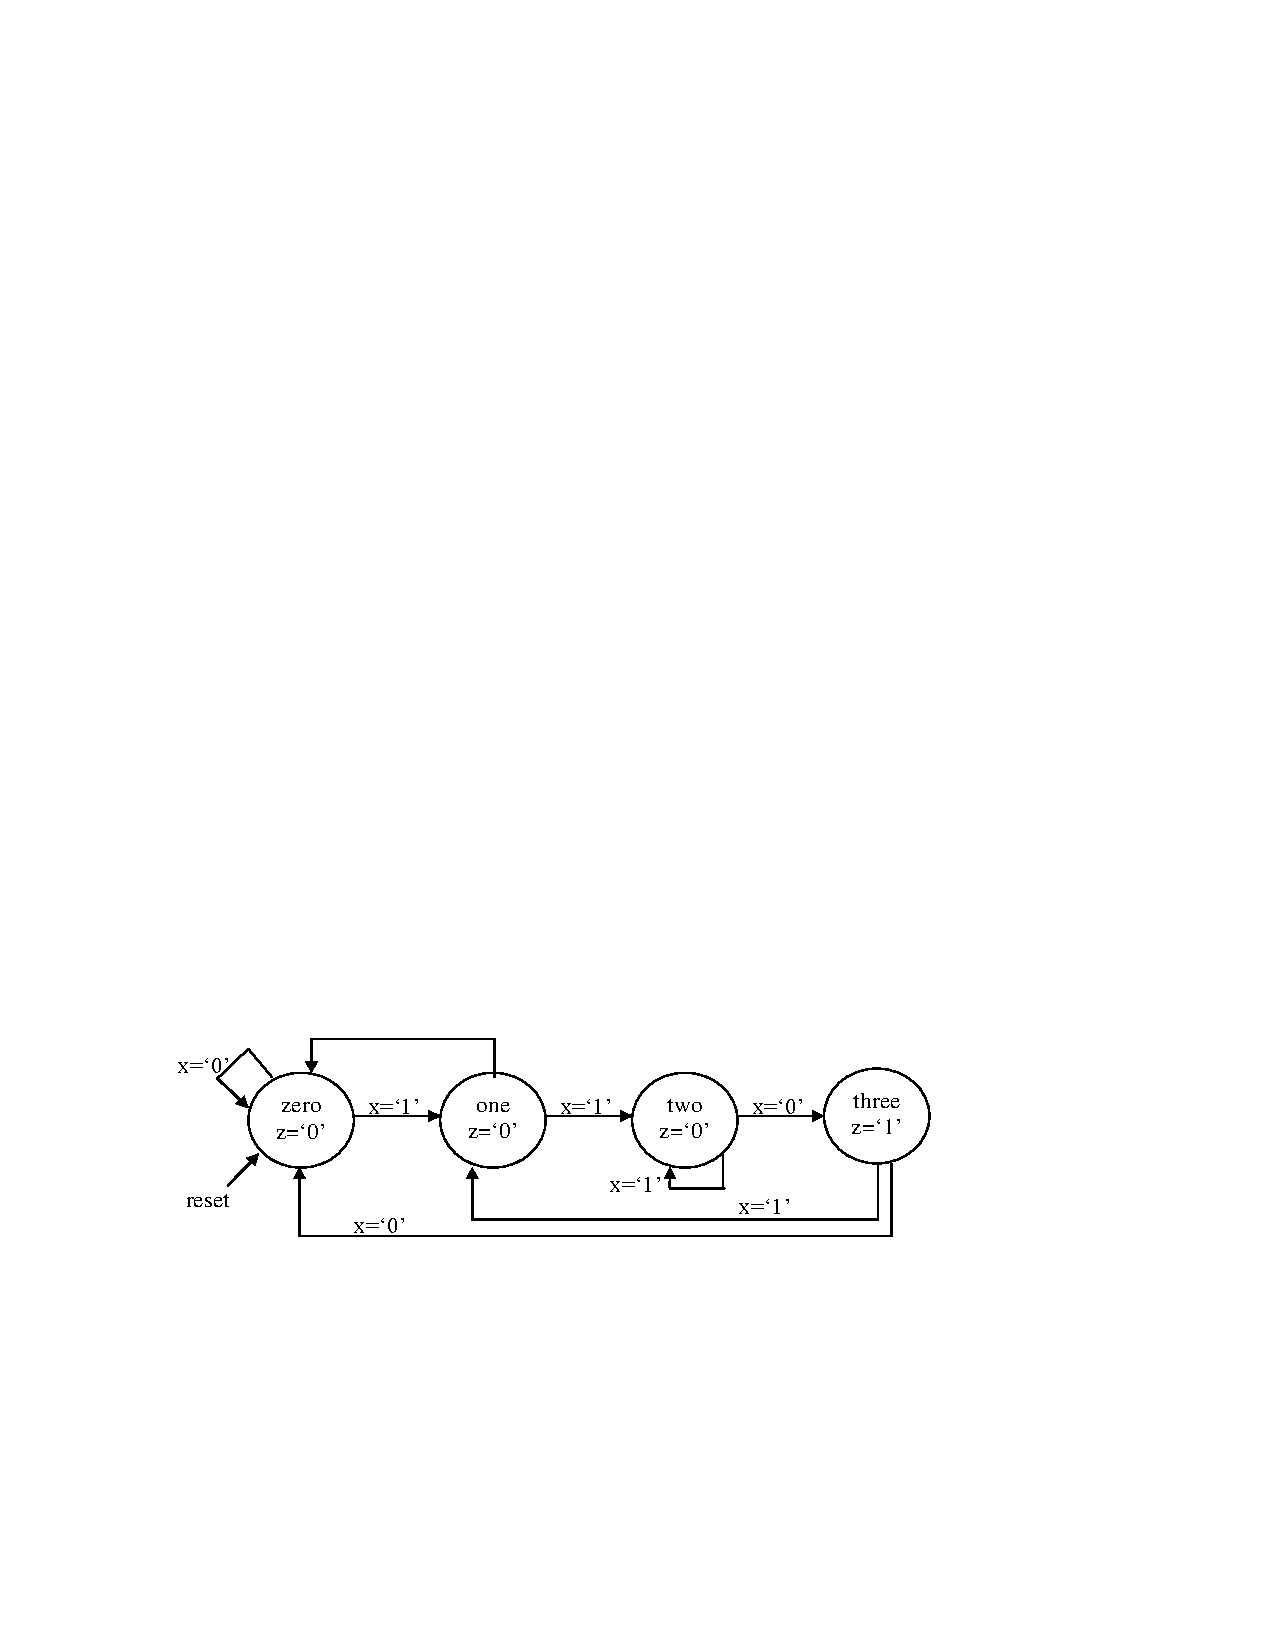
\includegraphics[width=1\columnwidth]{Moore_seq_det_state}
		\caption{Moore design}
		
	\end{subfigure} %  
	\begin{subfigure}[t]{0.5\textwidth}
		\centering
		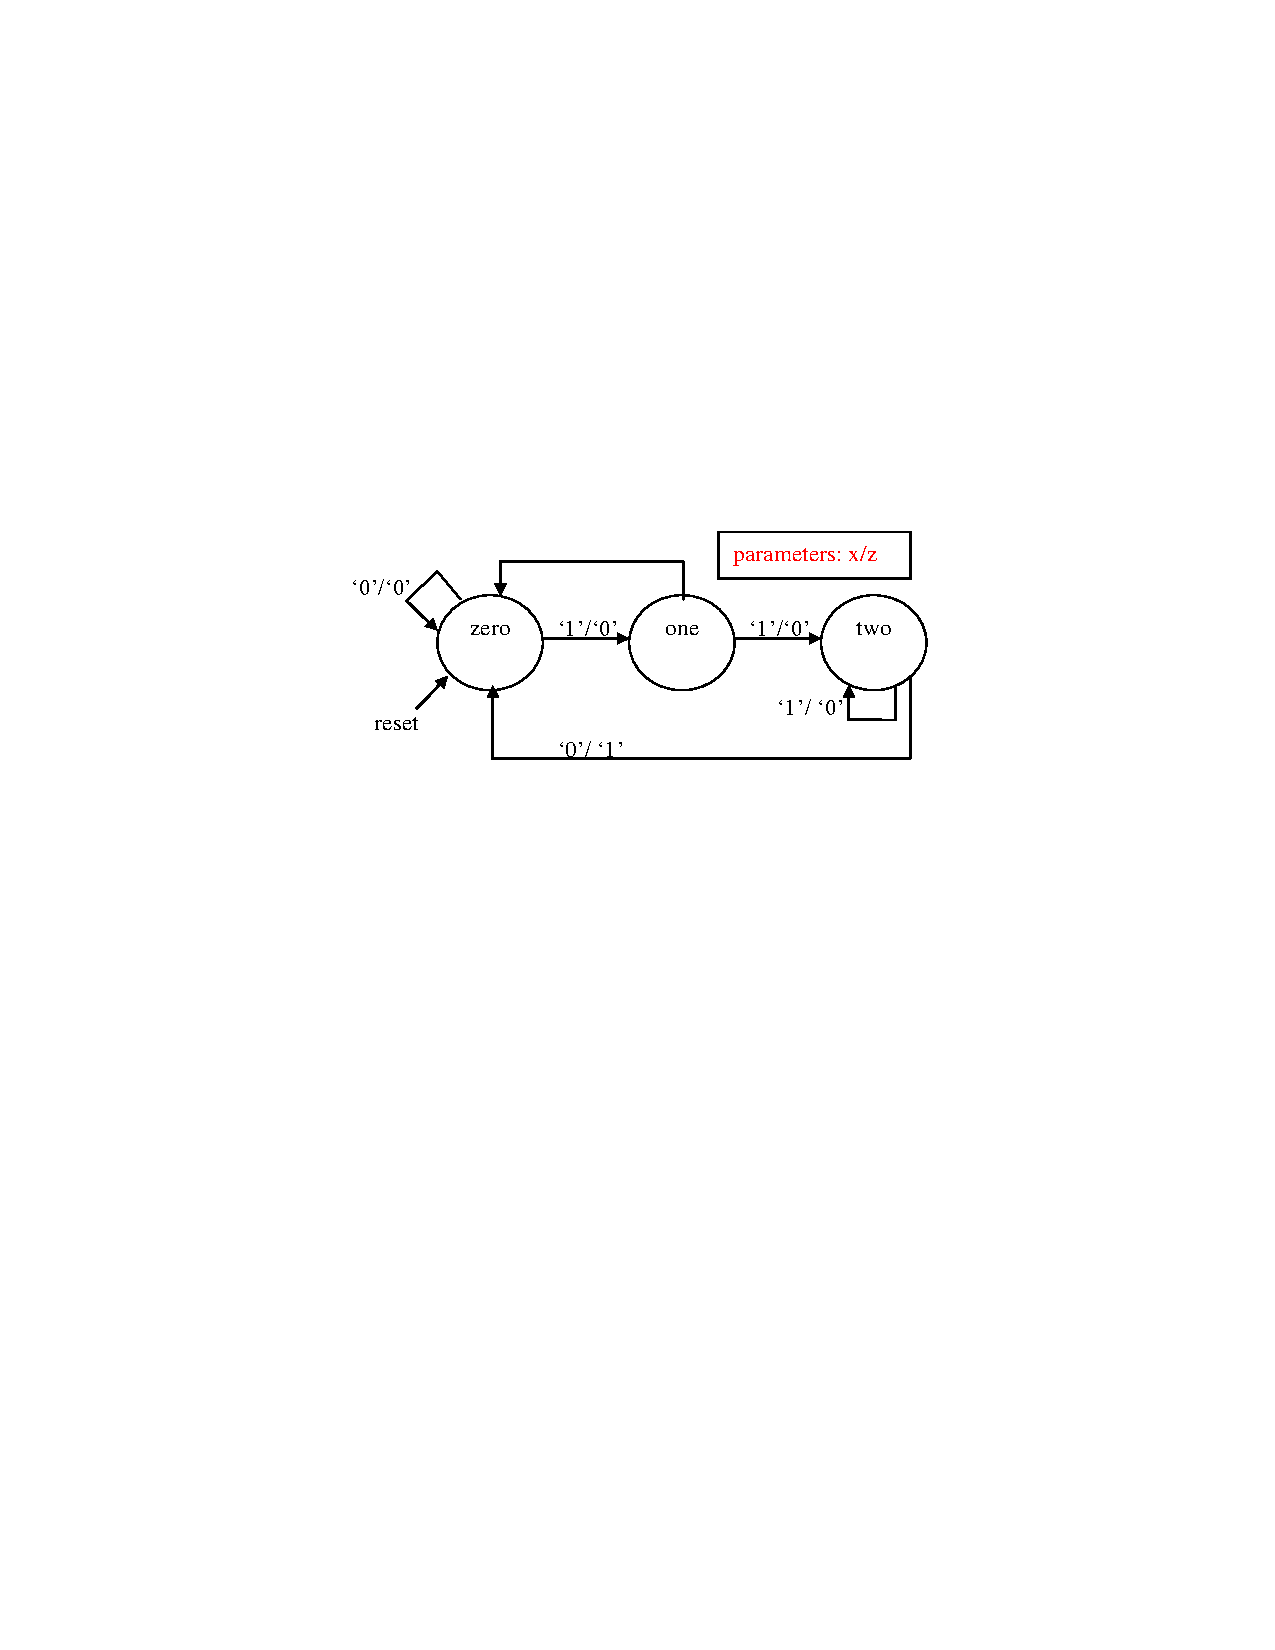
\includegraphics[width=1\columnwidth]{Mealy_seq_det_state}
		\caption{Mealy design}
		\label{subfig:Mealy_seq_det_state}
	\end{subfigure}		
	\caption{Non-overlap sequence detector : 110}
	\label{fig:non-overlap-design}%
\end{figure*}

\begin{figure}[!h]
	\centering
	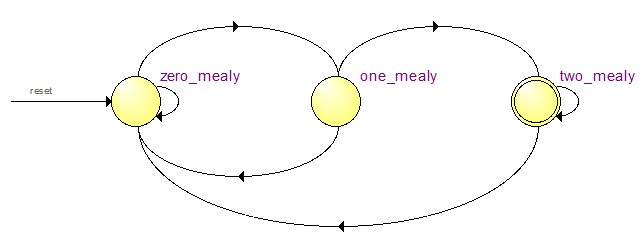
\includegraphics[scale=0.8]{Altera_Mealy_seq_det_state}
	\caption{State diagram generated by Quartus for Mealy machine in Listing \ref{verilog:sequence_detector}}
	\label{fig:Altera_Mealy_seq_det_state}
\end{figure}


\begin{figure}[!h]
	\centering
	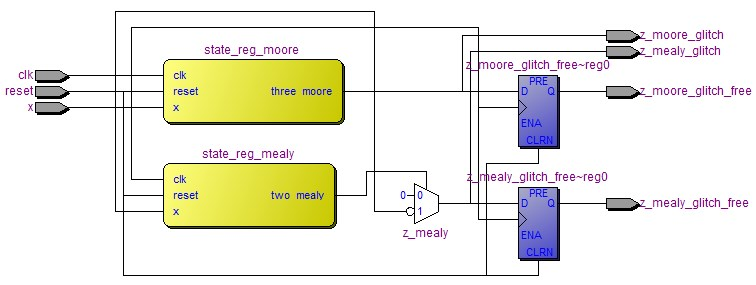
\includegraphics[width=\textwidth]{Mealy_Moore_RTL_glitchfree}
	\caption{RTL view generated by Listing \ref{verilog:sequence_detector}}
	\label{fig:Mealy_Moore_RTL_glitchfree}
\end{figure}

\begin{figure}[!h]
	\centering
	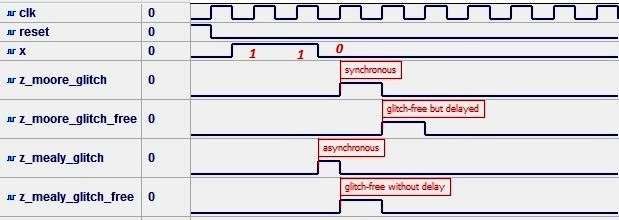
\includegraphics[width=\textwidth]{Mealy_MooreGlitchFree}
	\caption{Mealy and Moore machine output for Listing \ref{verilog:sequence_detector_tb}}
	\label{fig:Mealy_MooreGlitchFree}
\end{figure}

\lstinputlisting[
language = Verilog,
caption    = {Glitch removal using D-FF},
label      = {verilog:sequence_detector}
]{sequence_detector.v}

\lstinputlisting[
language = Verilog,
caption    = {Testbench for Listing \ref{verilog:sequence_detector}},
label      = {verilog:sequence_detector_tb}
]{sequence_detector_tb.v}


\subsection{Timed machine : programmable square wave }
Listing \ref{verilog:square_wave_ex} generates the square wave using Moore machine, whose `on' and `off' time is programmable (see Lines 6 and 7) according to state-diagram in Fig. \ref{fig:program_s_wave}.  The simulation waveform of the listing are shown in Fig. \ref{fig:square_wave_ex}.

\begin{figure}[!h]
	\centering
	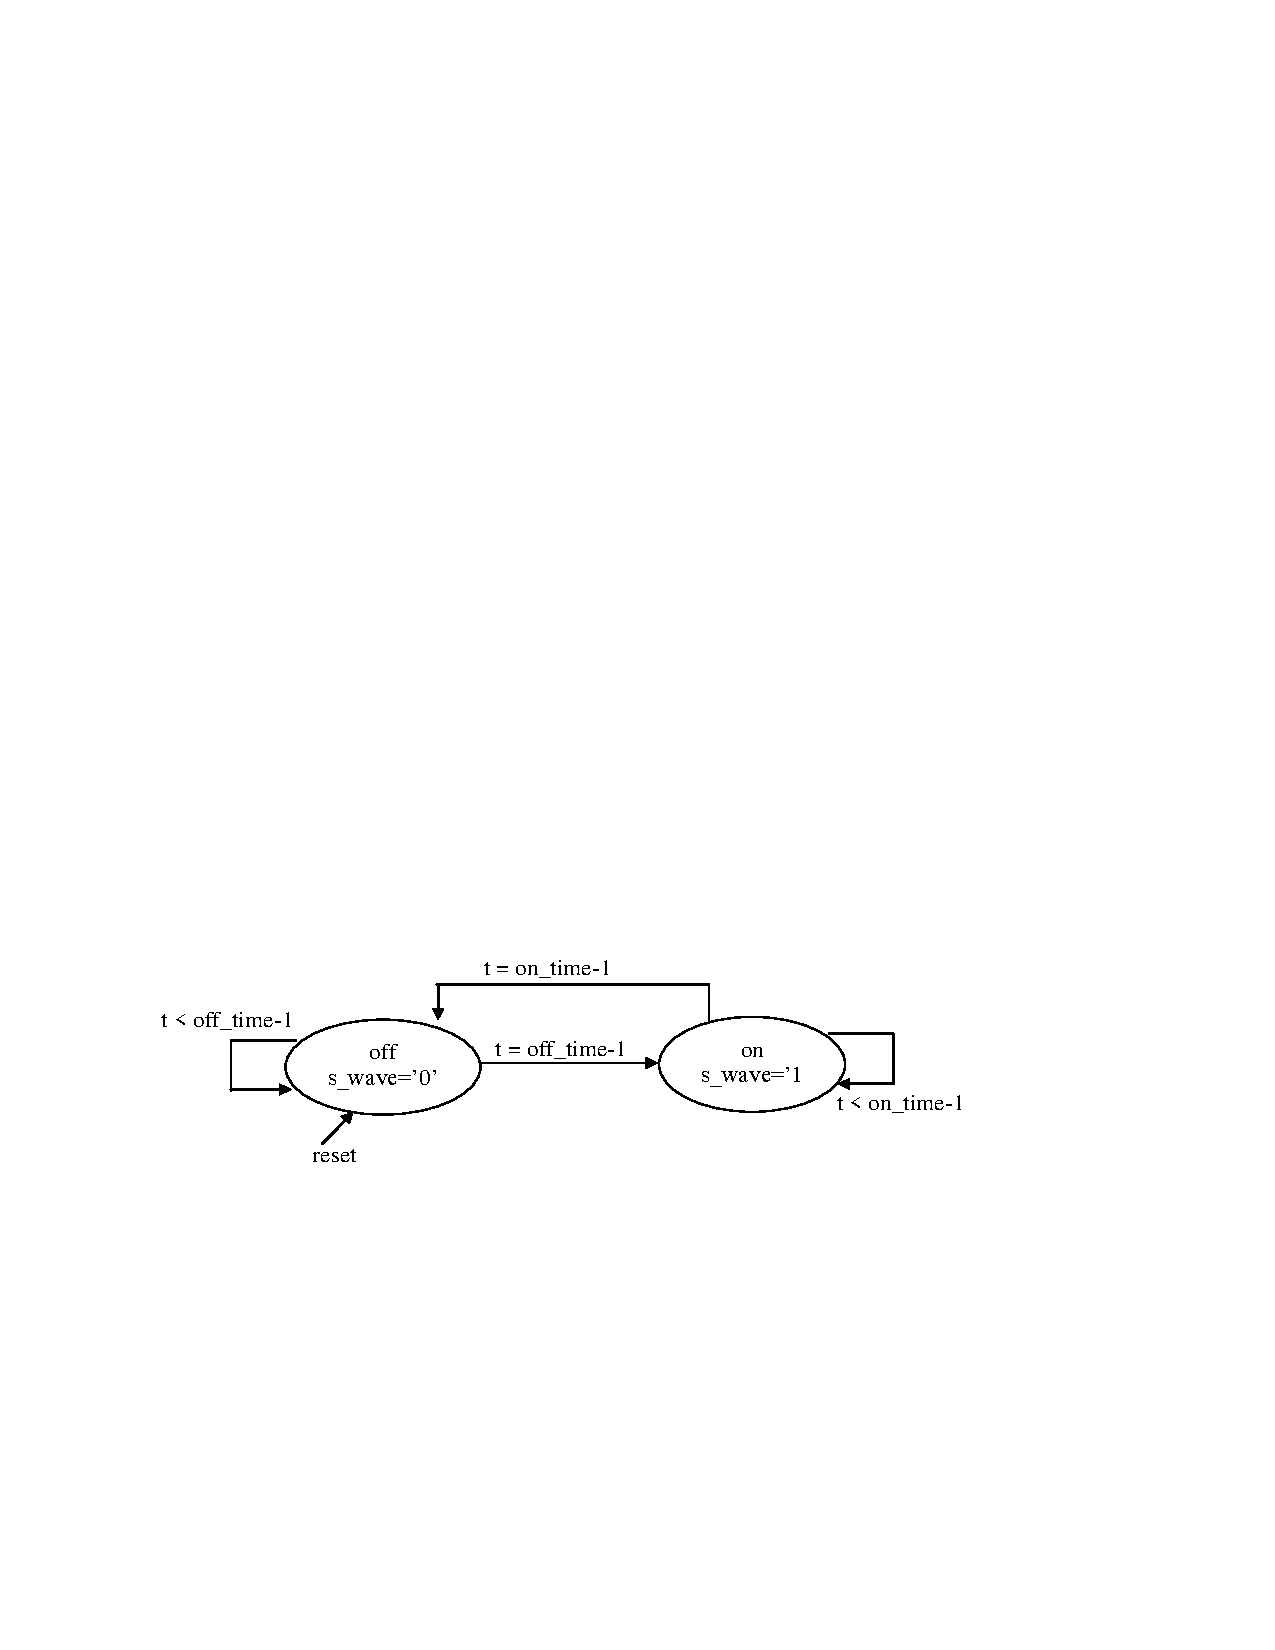
\includegraphics[scale=0.8]{program_s_wave}
	\caption{State diagram for programmable square-wave generator}
	\label{fig:program_s_wave}
\end{figure}

\begin{figure}[!h]
	\centering
	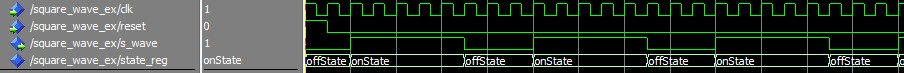
\includegraphics[width=\textwidth]{square_wave_ex}
	\caption{Simulation waveform of Listing \ref{verilog:square_wave_ex}}
	\label{fig:square_wave_ex}
\end{figure}

\lstinputlisting[
language = Verilog,
caption    = {Square wave generator},
label      = {verilog:square_wave_ex}
]{square_wave_ex.v}


\subsection{Recursive Machine : Mod-m counter}
Listing \ref{verilog:counterEx} implements the Mod-m counter using Moore machine, whose state-diagram is shown in Fig. \ref{fig:counter_state_diagram}. Machine is recursive because the output signal `count\_moore\_reg' (Line 50) is used as input to the system (Line 32). The simulation waveform of the listing are shown in Fig. \ref{fig:counterEx}

\begin{figure}[!h]
	\centering
	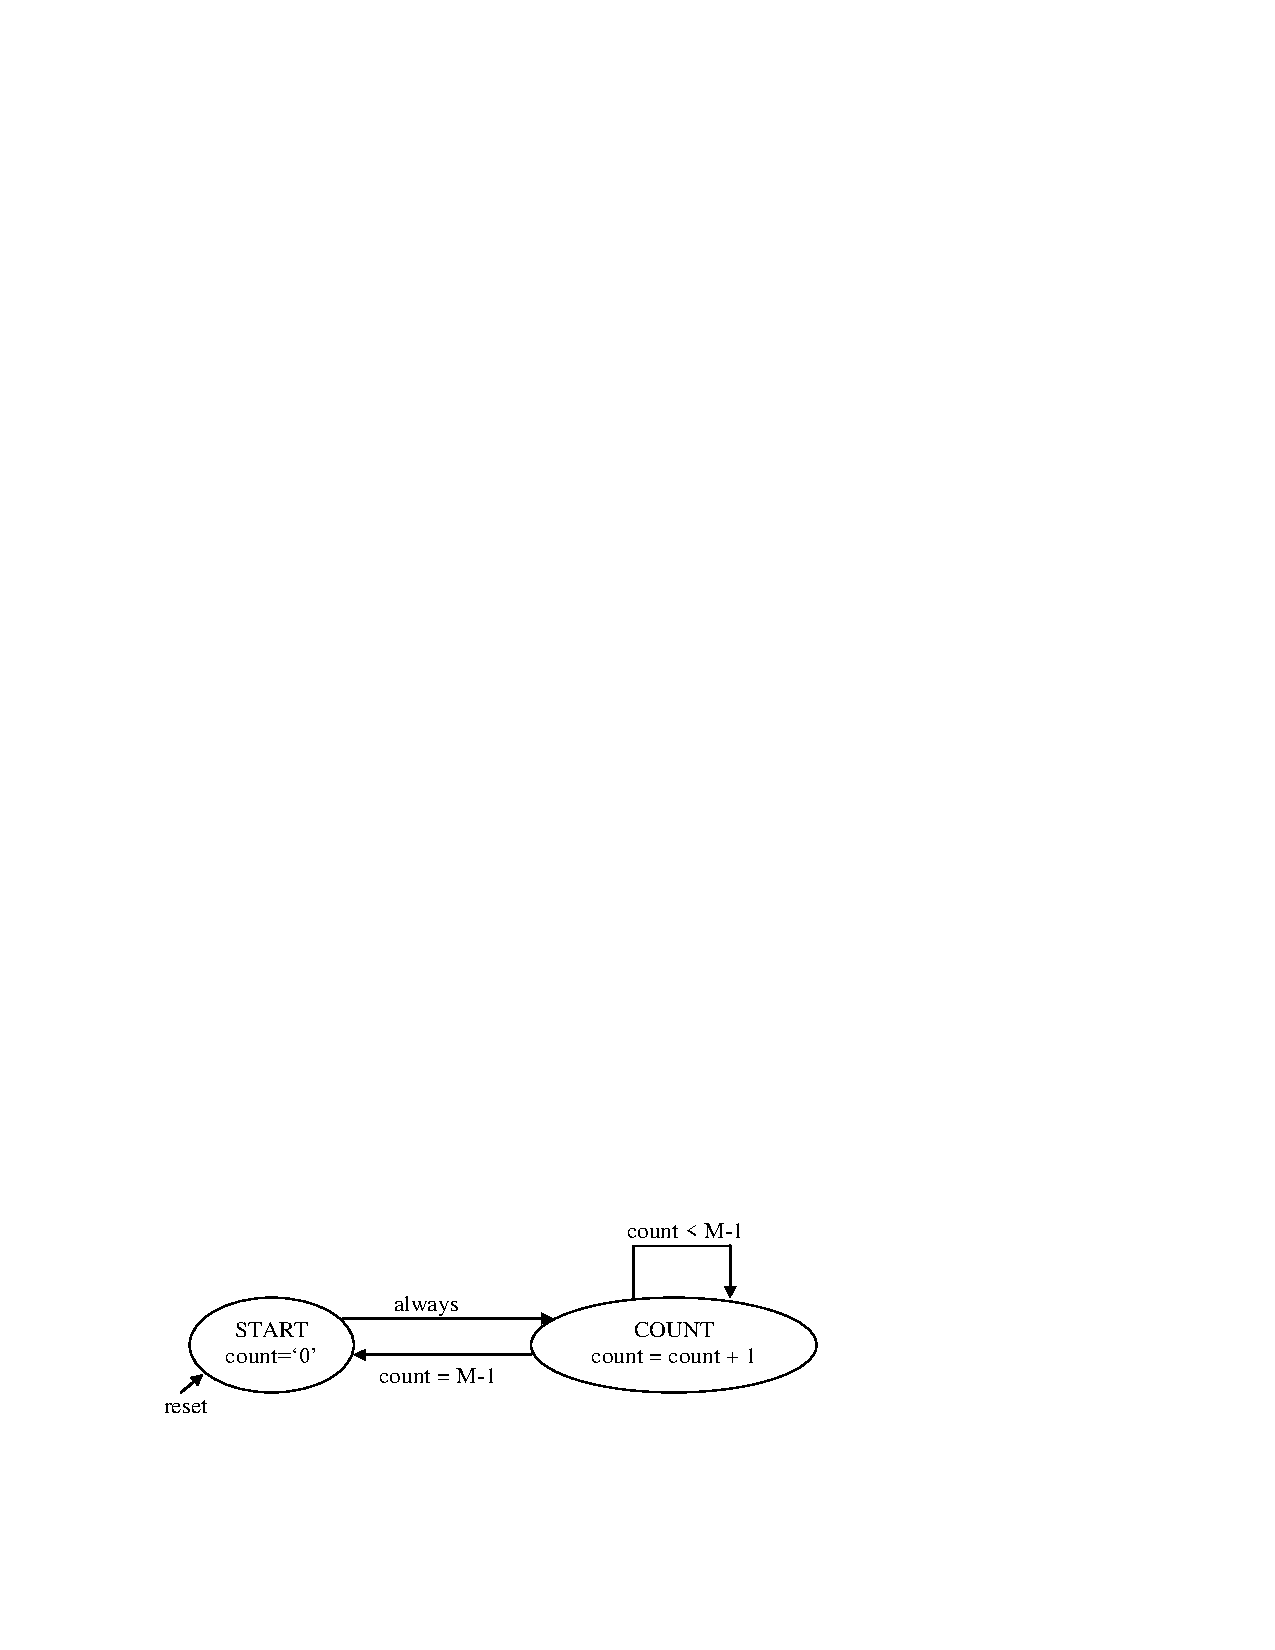
\includegraphics[scale=0.8]{counter_state_diagram}
	\caption{State diagram for Mod-m counter}
	\label{fig:counter_state_diagram}
\end{figure}

\begin{figure}[!h]
	\centering
	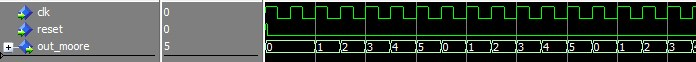
\includegraphics[width=\textwidth]{counterEx}
	\caption{Simulation waveform of Listing \ref{verilog:counterEx}}
	\label{fig:counterEx}
\end{figure}

\begin{noNumBox}
	It is not good to implement every design using FSM e.g. Listing \ref{verilog:counterEx} can be easily implement without FSM as shown in Listing \ref{verilog:modMCounter}. Please see the Section \ref{sec:whentouseFsm} for understading the correct usage of FSM design. 
\end{noNumBox}

\lstinputlisting[
language = Verilog,
caption    = {Mod-m Counter},
label      = {verilog:counterEx}
]{counterEx.v}


\section{When to use FSM design}\label{sec:whentouseFsm}
We saw in previous sections that, once we have the state diagram for the FSM design, then the Verilog design is a straightforward process. But, it is important to understand the correct conditions for using the FSM, otherwise the circuit will become complicated unnecessary. 

\begin{enumerate}
	\item We should not use the FSM diagram, if there is only `one loop' with `zero or one control input'. `Counter' is a good example for this. A 10-bit counter has 10 states with no control input (i.e. it is free running counter). This can be easily implemented without using FSM as shown in Listing \ref{verilog:binaryCounter}. If we implement it with FSM, then we need 10 states; and the code and corresponding design will become very large. 
	
	\item If required, then FSM can be use for `one loop' with `two or more control inputs'. 
	
	\item FSM design should be used in the cases where there are very large number of loops (especially connected loops) along with two or more controlling inputs. 
	
\end{enumerate}


\section{Conclusion}
In this chapter, Mealy and Moore designs are discussed. Also, `edge detector' is implemented using Mealy and Moore designs. This example shows that Mealy design requires fewer states than Moore design. Further, Mealy design generates the output tick as soon as the rising edge is detected; whereas Moore design generates the output tick after a delay of one clock cycle. Therefore, Mealy designs are preferred for synchronous designs. 

 